\documentclass[a4paper,12pt]{article}

\usepackage{fontspec} %note for JW: uncomment for XeLaTeX
\usepackage{xunicode} %note for JW: uncomment for XeLaTeX
\usepackage{textcomp} %note for JW: uncomment for XeLaTeX
\usepackage{graphicx} %note for JW: uncomment for XeLaTeX

\usepackage[english]{babel}

\usepackage{url}

\usepackage{colortbl}

\usepackage{subscript}

\usepackage{linguex}

\usepackage{qtree}

\usepackage{lscape}

\usepackage{longtable}

\usepackage{tabularx}

\setromanfont{Arial} %note for JW: uncomment for XeLaTeX

\usepackage{natbib}
\bibpunct[: ]{(}{)}{;}{a}{}{;}

\begin{document}
\urlstyle{same}
%\newfontinstance\scshape[Letters=SmallCaps,Numbers=Uppercase]{Hoefler Text}

%just temporary, for easier browsing the PDF
\tableofcontents
\newpage
%just temporary, for easier browsing the PDF

\begin{flushleft}
\begin{Large}
\textit{Funding Initiative\\
\textbf{“Documentation of Endangered Languages”}}\\\bigskip
\end{Large}

\textbf{VolkswagenStiftung}\\
Dr.\,Vera Szőllősi-Brenig\\
Kastanienallee 35\\
30519 Hannover\\
GERMANY
\end{flushleft}

\begin{flushright}
\today
\end{flushright}

\begin{flushleft}
\begin{tabularx}{\textwidth}{ l | X }
\hline
\multicolumn{2}{>{\large\columncolor[gray]{0.8}} c }{Personal data and adresses}\\
\multicolumn{2}{>{\large\columncolor[gray]{0.8}} c }{Applicant(s), cooperation partner, grant recipient}\\
\hline
\multicolumn{2}{>{\large\columncolor[gray]{0.8}} l }{Principal applicant}\\
\hline
\hline
\textbf{Family Name} & {\textbf{Trosterud}}\\
\hline
\textbf{First Name} & {\textbf{Trond}}\\
\hline
Female / Male & {Male}\\
\hline
Titel & {PhD}\\
\hline
Field of Study & {Saami linguistics}\\
\hline
\hline
\textbf{Institution} & {\bf{Universitetet i Tromsø}}\\
\hline
\textbf{Department} & {\textbf{Institutt for språkvitskap}}\\
\hline
Postcode & {9037}\\
\hline
City & {Tromsø}\\
\hline
Country & {Norway}\\
\hline
Phone No & {+47-77644763}\\
\hline
E-Mail Address & {trond.trosterud@uit.no}\\
\hline
Homepage & {http://www.hum.uit.no/a/trond/}\\
\hline
\end{tabularx}
\end{flushleft}

\noindent The application has not been / will not be submitted to other funding institutions.\\

Signature\\

\noindent \textit{\textbf{Please note that the Volkswagen Foundation – in accordance with regulations safeguarding data privaty – records electronically your personal data as well as the project proposal.}}

\newpage

\begin{flushleft}
\begin{tabularx}{\textwidth}{ l | X }
\hline
\multicolumn{2}{>{\large\columncolor[gray]{0.8}} l }{Co-applicant and grant recipient}\\
\hline
\textbf{Family Name} & {\textbf{Rießler}}\\
\hline
\textbf{First Name} & {\textbf{Michael}}\\
\hline
Female / Male & {Male}\\
\hline
Titel & {M.A. (Dr.\,phil expected 2010)}\\
\hline
Field of Study & {Scandinavian linguistics}\\
\hline
\hline
\textbf{Institution} & \textbf{Albrecht-Ludwigs-Universität Freiburg i.\,Br.}\\
\hline
\textbf{Department} & \textbf{Skandinavisches Seminar}\\
\hline
Street & {Platz der Universität 3}\\
\hline
Postcode & {79085}\\
\hline
City & {Freiburg}\\
\hline
Country & {Germany}\\
\hline
Phone No & {+49-761-203-3300}\\
\hline
Mobile Phone No & {+49-179-9441585}\\
\hline
Fax No & {+49-761-203-3366}\\
\hline
E-Mail Address & {michael.riessler@skandinavistik.uni-freiburg.de}\\
\hline
Homepage & \url{www.skandinavistik.uni-freiburg.de/institut/mitarbeiter/riessler/}\\
\hline
\end{tabularx}
\end{flushleft}

\newpage

\begin{flushleft}
\begin{tabularx}{\textwidth}{ l | X }
\hline
\multicolumn{2}{>{\large\columncolor[gray]{0.8}} l }{Co-applicant}\\
\hline
\textbf{Family Name} & {\textbf{Gerstenberger}}\\
\hline
\textbf{First Name} & {\textbf{Ciprian}}\\
\hline
Female / Male & {Male}\\
\hline
Field of Study & {Computational linguistics}\\
\hline
\hline
\textbf{Institution} & {\bf{Universitetet i Tromsø}}\\
\hline
\textbf{Department} & {\textbf{Institutt for språkvitskap}}\\
\hline
Postcode & {9037}\\
\hline
City & {Tromsø}\\
\hline
Country & {Norway}\\
\hline
Phone No & {+47-77644746}\\
\hline
E-Mail Address & {ciprian.gerstenberger@uit.no}\\
\hline
Homepage & {\url{http://www.hum.uit.no/a/gerstenberger}}\\
\hline
\end{tabularx}
\end{flushleft}

\newpage

\begin{flushleft}
\begin{tabularx}{\textwidth}{ l | X }
\hline
\multicolumn{2}{>{\large\columncolor[gray]{0.8}} l }{Co-applicant}\\
\hline
\textbf{Family Name} & {\textbf{Wilbur}}\\
\hline
\textbf{First Name} & {\textbf{Joshua Karl}}\\
\hline
Female / Male & {Male}\\
\hline
Field of Study & {Documentary Linguistics}\\
\hline
\hline
\textbf{Institution} & {\bf{Humboldt-Universität zu Berlin}}\\
\hline
\textbf{Department} & {\textbf{Nordeuropa-Institut}}\\
\hline
Postcode & {10099}\\
\hline
City & {Berlin}\\
\hline
Country & {Germany}\\
\hline
Phone No & {+49-30-2093-4850}\\
\hline
Fax No & {+49-30-2093-9626}\\
\hline
E-Mail Address & {wilburjk@staff.hu-berlin.de}\\
\hline
Homepage & {\url{http://www.ni.hu-berlin.de/personal/jwil/jwil_html}}\\
\hline
\end{tabularx}
\end{flushleft}

\newpage

\section*{Project proposal}

\section{Basic information}

\begin{tabbing}
LLLLLLLLinks \= Mitte \= Rechts \kill
Project title: \>\textbf{Language Technology for Small Saami Languages}\\
%alternative titles:
%Multimedia corpora and language technology for highly endangered Saami languages
%Computer-aided analyses of Saami language corpora
%Spoken corpora and computational linguistics for small Saami languages
Total budget: \>\textbf{300,000 €}\\
Project period: \>\textbf{August 2011 – July 2014}\\
\end{tabbing}
Keywords: {\it Documentary Linguistics, Saami Linguistics, Computer Linguistics, Applied Linguistics, Corpus Linguistics, Revitalization; Kildin Saami, Ter Saami, Ume Saami, Pite Saami, ISO 639-3: sje, sjd, sjt, sju}

\section{Abstract}%up to 2 pages /finished, but has to by checked for consistency before finalizing the application 
The proposed project will use existing DoBeS and ELAR archives to create a state-of-the-art corpus infrastructure as well as language technology tools for four endangered Saami languages: Ume, Pite, Kildin and Ter Saami. This shall involve a variety of aspects relevant to the field of modern documentary linguistics: endangered language documentation and archiving practices, automatic annotation, and computer-aided tools for creating lexica and educational materials. Ultimately, the project intends to develop new methods for processing already extant archived linguistic data from endangered Saami languages in order to improve subsequent/future corpus linguistic research and to support language revitalization efforts with language technology.

The main goal of the project is twofold: 1) to apply language technology tools to efficiently supplement corpora of digitized, transliterated and translated texts with consistent annotations, and 2) using the resulting annotated corpora, to then create practical applications such as paradigm and word-form generators, interactive teaching materials and electronic lexica. As a result, the needs of both the academic community and the speech communities concerned will be served.

Specifically, the project shall result in the following outcomes: 1) a searchable corpus of spoken language for these four endangered Saami languages which shall be linked to multimedia files and intended not only %particularly 
for use in linguistic research, but also as a gateway to the corpus for the language communities; 2) semi-automatic annotation of the corpus; 3) implementing language tools for both linguists and revitalization activists such as lemmatizers, part-of-speech
  taggers, dependency parsers, 
 (online/offline) electronic dictionaries, translation tools, educational materials, etc. %(again based on tools currently used by Giellatekno for North Saami)
 ; 4) development of methods, workflows, conventions and best-practice guidelines for such projects; and
5) dissemination of these outcomes to be utilized in the future as at least a template or source of inspiration for other DoBeS, ELAR and other endangered language projects for developing corpus linguistics and language technologies.

Pite Saami and Ume Saami are spoken in Sweden, while Kildin Saami and Ter Saami are spoken in Russia; they belong genealogically to distinct subbranches of the Saami group inside Uralic: Ume is in the southern branch of West-Saami, Pite in the central branch of West-Saami, and Kildin and Ter belong to the Peninsula branch of East-Saami. All four languages are highly endangered or moribund due to ongoing language shift to the regional suprastrate Indo-European languages Swedish and Russian.

For three of the four languages in question, annotated multimedia corpora already exist thanks to the groundwork carried out by principle applicant Michael Rießler (partially with the help of co-applicants E.\,Karvovskaya and J.\,Wilbur) for the Kola Saami Documentation Project (a DoBeS project) and by co-applicant J.\,Wilbur for the Pite Saami Documentation Project (a Hans Rausing Endangered Languages Project). These corpora covering Kildin, Ter and Pite Saami will form the initial core set of resources for the project's work, but will be supplemented with more data and more elaborate annotations in the course of the project, as well as with addition of the first annotated corpus of Ume language materials. While automatic generation of annotations and corpora is nothing new, the application of such computer-aided technologies to spoken, multimedia archived materials of endangered languages is a first.

Community-driven revitalization efforts are underway to varying extents for all four languages. Thus, there is local interest in working on these languages while speakers are still living, and the proposed project will work closely with the language communities in producing practical products in tune with the respective communities' wishes and expectations.

The project will be carried out within the framework of contemporary documentary linguistics and as a joint effort between the Scandinavian Department at Freiburg University and the center for Saami language technology (Giellatekno) at the University of Tromsø.
The team shall consist of experienced documentary and computational linguists as well as programmers, all of whom are familiar with Saami languages in general and have excellent working knowledge of the Saami languages in question and the relevant \textit{lingua franca}. Team members are also well versed in corpus- and computational linguistics, in carrying out documentation fieldwork, and in practical revitalization issues. The project will also profit from the symbioses already in place between researchers familiar with the Giellatekno infrastructure (including tools for other northern languages) and researchers acquainted with the DoBeS and ELAR infrastructures (documentary linguistics of spoken language, archiving of annotated multimedia).

The two leaders of the project are documentary linguist Michael Rießler (Freiburg) and computational linguist Trond Trosterud (Tromsø), both of whom are specialized in Saami linguistics. The first applicant is a junior researcher who also led a DoBeS project on the Kola Saami languages. The other two applicants are Joshua Wilbur, currently coordinator/researcher for the Pite Saami Documentation Project (ELDP), and Giellatekno's programmer Ciprian Gerstenberger. Funding for the proposed project would go towards a full principle researcher position for M.\,Rießler and a half-time principle researcher position for J.\,Wilbur at the University of Freiburg, two student research assistants as well as material support and travel expenditures.

%\begin{figure}[h]
%\begin{center}
%\caption{S\'{a}pmi and the Saami languages. The languages of the project are ??} 
%\label{SaamiLgs}
%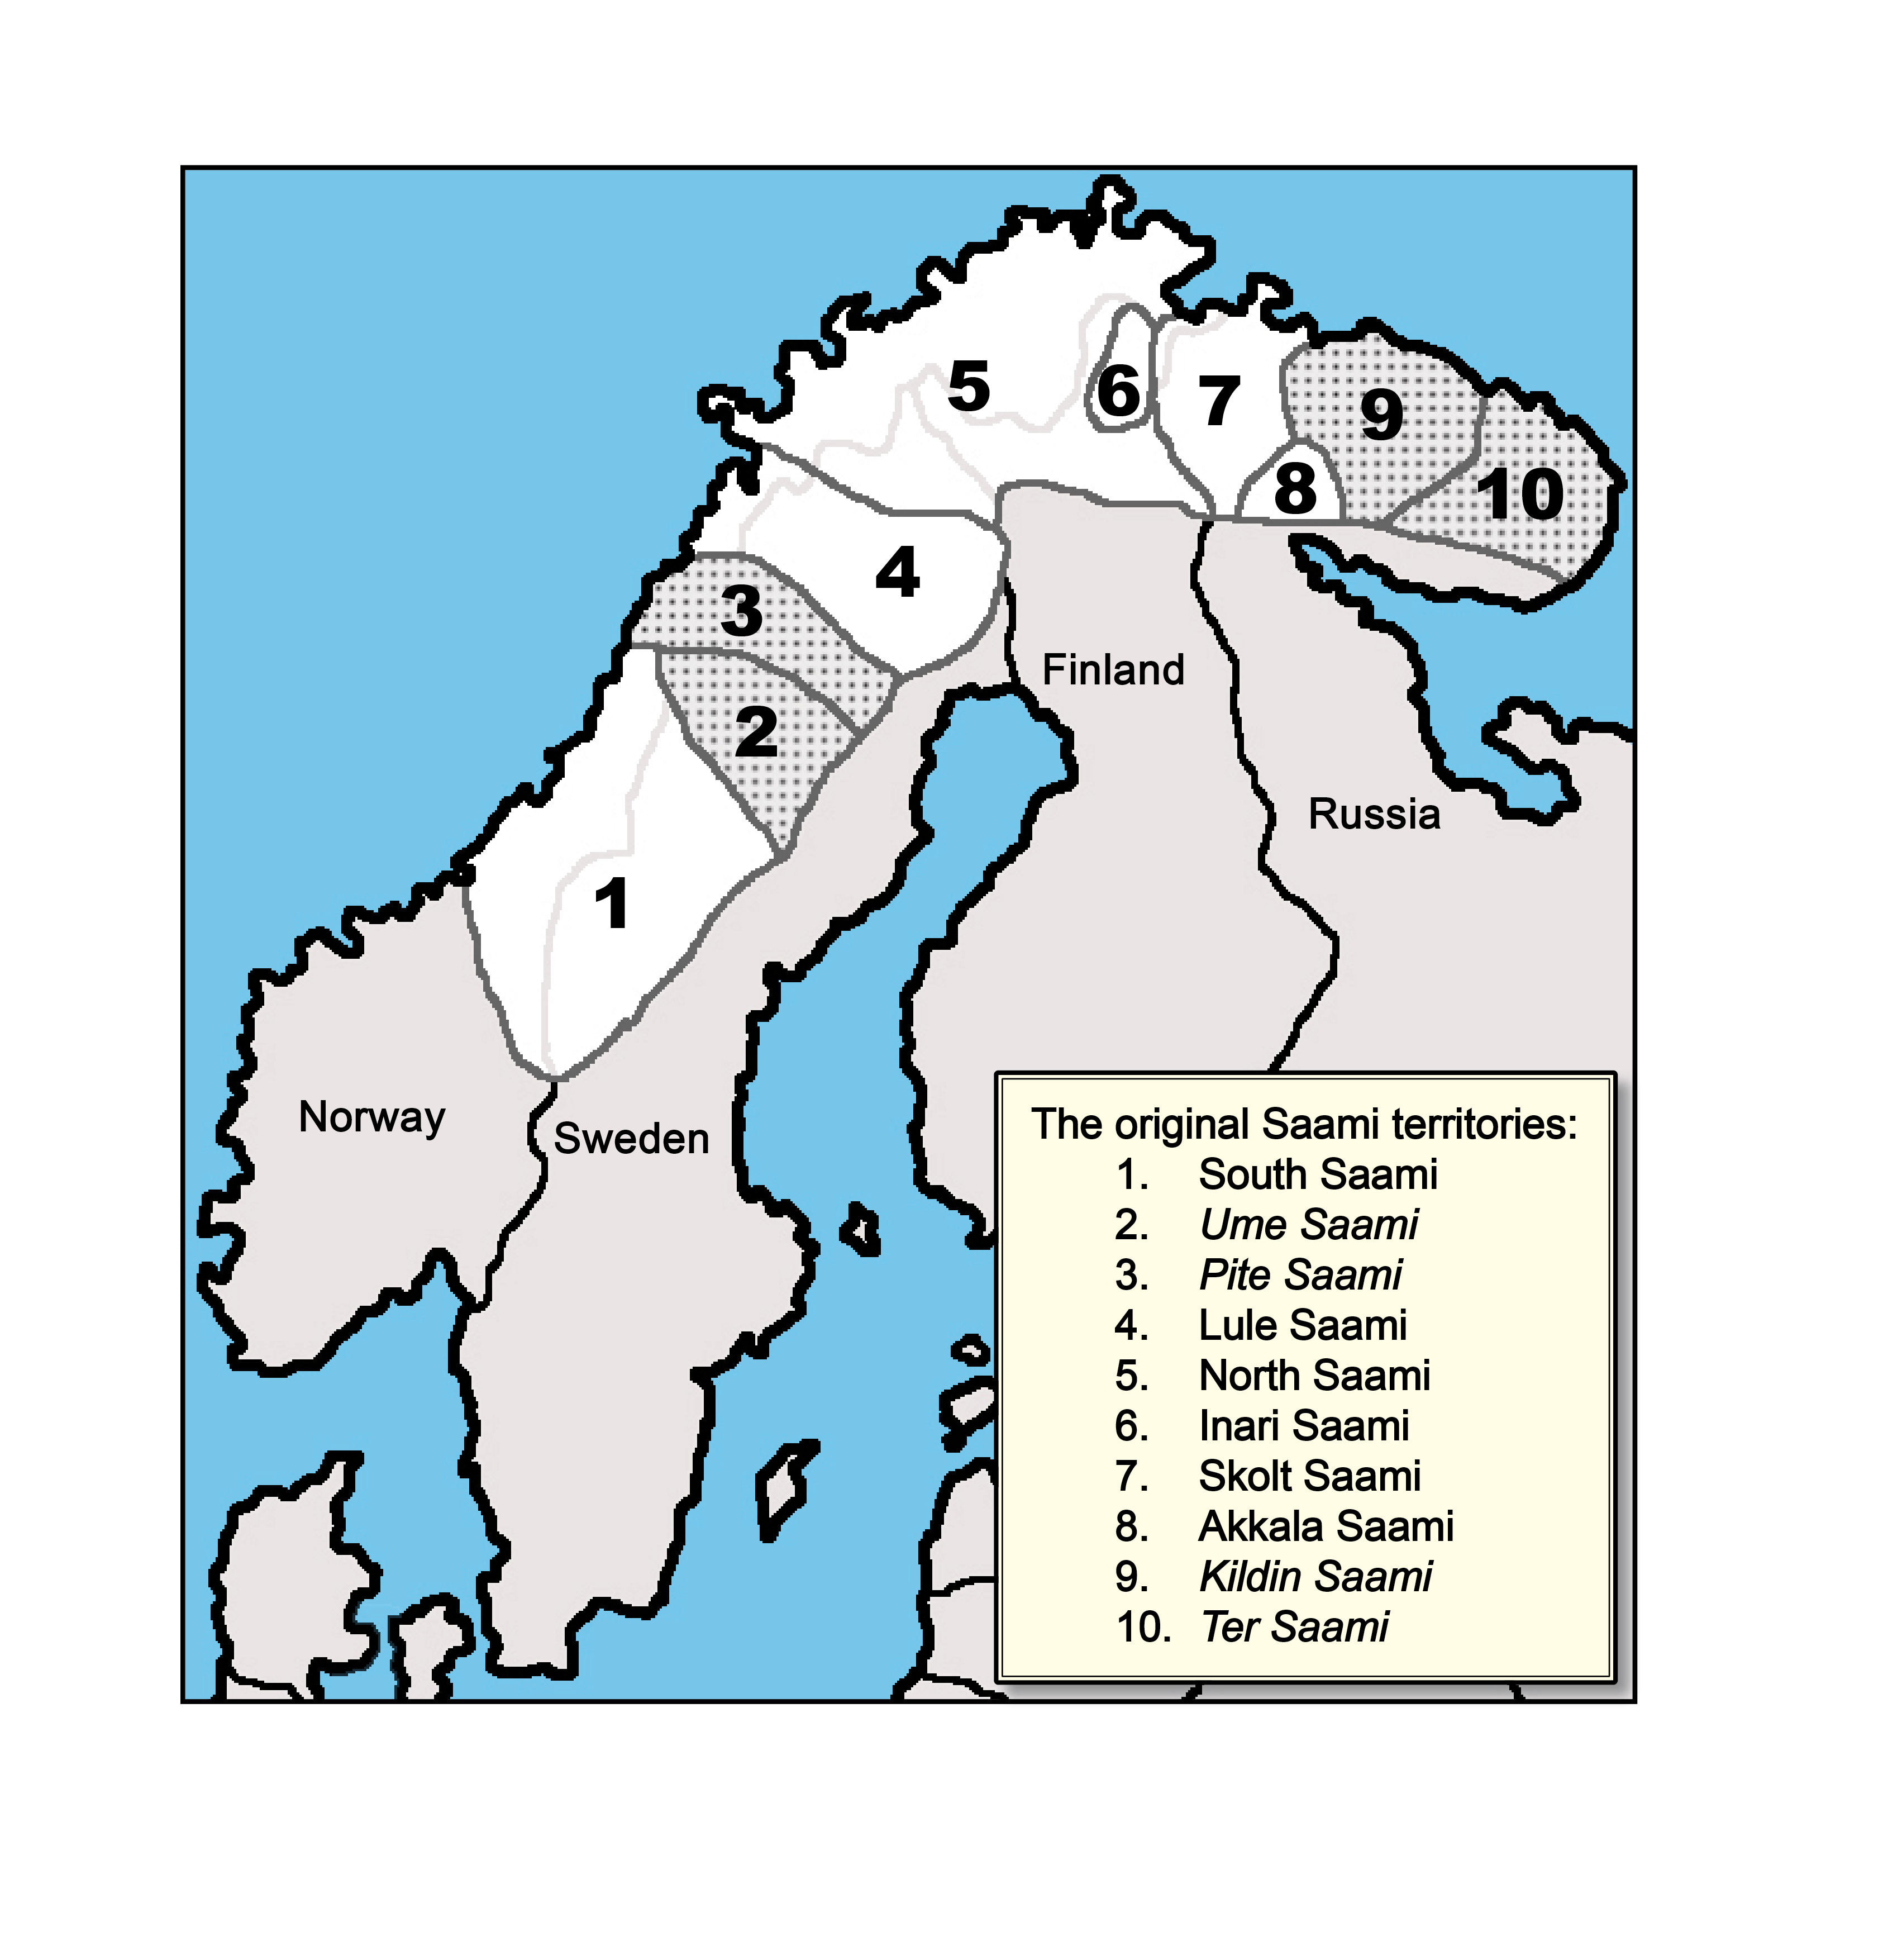
\includegraphics[width=0.9\textwidth]{SaamiLgs.jpeg}
%\end{center}
%\end{figure}

\section{Detailed project description}%up to 25 pages
\subsection{Introduction}

The \textit{Dokumentation bedrohter Sprachen} (DoBeS) and the \textit{Hans Rausing Endangered Language Project} (which ELAR is a part of) programs have the aim to create data-orientated, multifunctional, and generally accessible documentations of endangered languages in order to support languages in danger of extinction and to help protect endangered linguistic and other cultural data from disappearing. In this, archiving recordings of spoken languages alone is not considered sufficient; instead, archived recordings must include metadata and annotations describing their contents. This should at least consist of cataloging metadata (concerning e.g. participants, recording location, etc.) and transcriptions of the recordings with translations into a stable \textit{lingua franca}. However, annotations can provide much more detailed information, such as the specifics provided by detailed linguistic analyses\footnote{Detailed linguistic analyses typically contain such information as part of speech, glosses, and/or word or morpheme boundaries.}. Such analyses are interesting and useful in and of themselves for linguistics research, but they also can be utilized to produce lexica, translation tools and teaching materials for use by linguists and, at least as important, by the relevant endangered language community. However, producing such detailed analyses is exceptionally time and resource consuming, and as a result, only a portion of archived materials typically include such detailed information. Fortunately, with the help of current computer-based technology, the availability of such detailed linguistic analyses in a computer-readable format can result in:
\begin{itemize}
\item easier and more effective searches of documentation corpora for both corpus linguists and language community members, including linking search results to the actual primary recordings;
\item the creation of lexica, translation tools and educational materials utilizing modern web-based technologies.
\end{itemize}
It is thus the logical next step from the perspective of both language and research communities to supplement archived materials with as much detailed linguistic analyses as possible and then, with the help of computers, to create practical products as a result. This task is particularly urgent for endangered languages because 1) access to native speaker knowledge is limited and potentially no longer possible in a relatively short time, and 2) because those involved in revitalization efforts want to take advantage of the practical tools that result in counteracting wide-spread language death at a local level as soon as these become available.

\subsection{Preliminary considerations}%almost finished, some formulations and the English are unfinished though
\paragraph{What are corpora?} In principle, any collection of language data is a corpus. However, depending
on the purpose of data collection, the raw, i.e. unannotated,  data is preprocessed and annotated accordingly. This means also that all transcriptions of recorded texts result in searchable corpora. If at least one translation is provided with the transcription, then it is a parallel corpus. However, most parts of Saami language documentation work are currently available as parallel corpora in books or other printed media and are thus only searchable manually. If such text corpora are scanned using text-recognition software (OCR, Optical Character Recognition), they can be made machine-readable, but the results can still be used only for raw text searches. In accordance with the central aims of contemporary documentary linguistics, i.e. data orientation, multi-functionality and general accessibility, DoBeS corpora (similar to ELAR or other archives) do not only provide a direct link to the original recordings but in most cases these corpora include independent linguistic (and even other non-linguistic) annotation. Normally, these annotations are created as the result of tedious manual labour or by using semi-automatic (morphological) parsers like Toolbox.

For languages with good access to informants and even native linguists, there is always the possibility of introspection and informant elicitation. Elicitation and introspection of data always run the risk of being influenced by the research situation, corpus data are gathered independent of the linguistic problem at hand, and therefore example of genuine language use. Also corpus data face methodological problems, though: Corpora are problematic when investigating non-existent and marginal forms.  For endangered, let alone extinct languages, corpus studies are the only empirical foundation available. In order to enable also future generations to investigate the languages in question, large and diverse corpora are needed.

\paragraph{What is corpus linguistics?} Corpus linguistics refers to the study of linguistic phenomena as expressed in real world texts such as in the printed text representations mentioned above, or in machine-readable corpora, which allows for much more efficient corpus research. One significant problem when trying to create a “quality” machine-readable corpus is keeping annotation standards consistent; this includes reserving one type of information for each annotation tier (e.g. part-of-speech in one tier, glosses in another tier), consistent use of certain tags or symbols for similar phenomena (e.g. sticking to a set list of morphological glosses, to a set method of morpheme boundaries, defined marking of non-linguistic phenomena, etc.). As opposed to pure manual annotations – which are mistake-prone, semi-automatic annotation methods using software such as Toolbox allow for more consistent tagging, at least in theory. However, in practice, some corpora stemming from Toolbox projects are only really searchable using a full text search due to inconsistent tagging and comprising several different kinds of information (e.g. phonological, morphological and morpho-phonological) into one and the same annotation tier. As a result, searching the content of such corpora is relatively limited.

To allow for a multi-layered, consistent annotation of linguistic data, the use of off-the-shelf annotation tools (e.g., NITE XML, MMAX, UAM CorpusTool, MATE Annotation Workbench, etc.) is indispensable. However, the idiosyncratic socio-cultural development of each Saami language poses challenges for building language corpora and making them work with annotation and searching tools. To choose and adapt such annotation tools for languages with peculiar writing systems, e.g. Kildin, is a non-trivial task. The present project aims at choosing and adapting such tools for the appropriate language representation for the languages under discussion. % a bit short, hmm
% yes, manual anotation may be inconsistent, but usually it is seen as gold standard
% thus, a more serious (?) problem is the workload involved in tagging large corpora, 
% compared to doing it automatically.

\paragraph{What are computational linguistics and language technology?} Computational linguistics refers to machine-based processing of natural language. This normally includes, among other things, the development of processes for the analysis and generation of natural language texts, programs to collect and statistically evaluate large amounts of language data (such as lemmatizing software, frequency wordlists, concordances). Computational linguistics also eases the process of building corpora mostly by using automated processes (typically morphological and syntactic disambiguation). A further goal for computational linguists is to build models of natural language grammars. When tested against actual language data, the models function as hypotheses for the form of the grammars in question. 

Language technology could be considered to be a (functional) application of computational linguistics as it is aimed at analyzing and generating natural language in various ways and for a variety of mostly practical purposes. Machine-based translation or computer-based language instruction are two examples of such practical applications.
 
\paragraph{What are multimedia spoken vs. written corpora?}
The Giellatekno group in Tromsø already has the know-how and the infrastructure necessary to deal with the above aspects of corpus and computational linguistics, and has fully implemented this for North Saami, as well as partly for Lule Saami and South Saami, and even some initial work for Kildin Saami. However, these are all written languages and the text corpora which Giellatekno's work has been based on have also been in written form (as mono-lingual or parallel texts with translations). The proposed project intends to take advantage of Giellatekno's experience and expand its field of application exclusively to spoken corpora. In theory, the input for the computational linguistic applications will be the same, since the spoken texts will first have to be represented as text (ortho-)graphically. However, there are several important aspects to consider in this (cf.~below Section \ref{method}).

Furthermore, many corpora are exclusively represented in writing, including the existing Giellatekno corpora. The proposed project, in focusing on spoken-language texts, will include links to the time-aligned multimedia recordings that the orthographic representations which make the corpora originate from. In and of itself, this is also nothing new. However, the corpora resulting from the proposed project will be linked to multimedia sources and include annotations done by semi-automatic morphological and syntactic parsing. In this, we will be joining documentary linguistics on endangered languages with corpus linguistics and with language technology. It is precisely these considerations which are at the source of motivation for the proposed project. As such, one of our main goal is to create a corpus linguistic infrastructure as a foundation for future Saami linguistic work using the DoBeS and ELAR materials. The other main goal being practical tools for aiding revitalization.

\paragraph{Why specifically these four Saami languages?}%Josh-diesen Absatz bitte nochmal ansehen!!
There are a variety of reasons why precisely these four Saami languages have been chosen to be the focus of the project. First of all, the depth and detail of annotations for archived endangered language materials for these Saami languages will be expanded. Second, the work going into creating automatic parsing tools will also be used to create practical language tools, which in turn will support current revitalization efforts by the respective language communities. Third, it is both sensible and practical to adapt Giellatekno experiences with North Saami\footnote{Specifically, this includes the computational linguistic infrastructure which is already in place for written North Saami as well as the computational linguistic know-how derived from dealing with monolingual and parallel written North Saami corpora.} to related Saami languages rather than starting from scratch. Fourth, these four Saami languages display interesting variation between each other %as well as within dialects of the individual languages%MR: ich meinte was anderes:
 in regard to their (quantitative and qualitative) state of documentation and to the degree they are ??verschriftlicht??. This allows for complex and rewarding methodological comparisons. Last but not least, the tools, workflows, experience and guidelines resulting from the project shall be able to be used as a kind of example or template for other projects working with language technology and/or corpora of endangered spoken languages.

%JW: ich finde diesen Abschnitt ziemlich schwach, weiß aber gerade nicht, was ich sonst schreiben soll. 
%MR: ich wollte hier erklären, warum genau diese kombination der vier saamischen Sprachen mit so unterschiedlichen Voraussetzungen total supertoll ist, um die wissenschaftliche Erkenntnis voranzubringen... 
%JW: ist jetzt hoffentlich besser.

\subsection{Urgency of documentation}\label{urgency}
The Saami languages (Uralic) form a dialect continuum across an area extending from central Scandinavia to the Kola Peninsula in the Russian Federation. Traditionally, the Saami were half-nomadic peoples who migrated annually between summer and winter settlements and survived on hunting and fishing. Herding reindeer was not a typical occupation until relatively recent times, but has become so at least in the central mountainous areas of Sápmi; nowadays all Saami live modern lives and blend in with the rest of the predominantly non-Saami population. Due to the influence of North Germanic, Finnic and Russian languages and cultures, all ethnic Saami are fluent in their respective contact languages, while younger generations are typically monolingual in these. As a result, the Saami languages are today either extinct, moribund or endangered. The least endangered Saami language is North Saami with not more than 17,000 speakers in Norway, Sweden and Finland \citep[1]{sammallahti1998b}.

\begin{figure}
\caption{Saami language tree} \label{saami tree}
\qtreecenterfalse
\Tree [.Saami [.{West Saami} [.South South Ume ] [.Central Pite Lule North ] ] [.{East Saami} [.Mainland Inari Skolt ✝Akkala ] [.Peninsula Kildin Ter ] ] ]
\end{figure}

The proposed project will focus on four particularly endangered Saami languages, as summarized here:
\begin{itemize}
\item Kildin (highly endangered, with an orthography, with some description and documentation)
\item Pite (moribund, without an [established] orthography, with little description and documentation)
\item Ter (moribund, without any orthography, with little description and documentation)
\item Ume (practically extinct, without an [established] orthography, with very little description and documentation)
\end{itemize}

Ume is a southern Saami language of West-Saami and spoken in central Swedish Lapland in and around the modern towns of Arvidsjaur, Malå, Ammarnäs and Tärna. Today, Ume is practically extinct, as the estimated number of speakers is less than five.\footnote{This is co-applicant J.\,Wilbur's own estimate, based partly on hear-say, and consists of one elderly woman in Lycksele, one man (approx. 40 years old) who taught himself Ume as a second language, but speaks it with his two children, who could be considered Ume speakers; according to J.\,Wilbur's contacts in Arjeplog, there are also two or three elderly non-active speakers in Arvidsjaur, Sweden.} Although the first Saami language book ever was a new testament bible translation in Ume Saami from 1755, no standardized orthography has been developed, nor is there any significant set of literature in Ume. However, one Ume language activist has recently developed some educational materials and texts on his own.

The situation for Pite Saami is not quite as desperate, but can hardly be described as positive. Pite (also known as Arjeplog Saami) is in the central branch of West-Saami and is currently spoken by approximately 30 speakers in and around the community of Arjeplog in central Swedish Lapland. Of these speakers, the vast majority are 50 years old or older and have neglected to teach their children Pite. There is one exception, a 33 year old reindeer herder who actively speaks Pite on a daily basis in his work with his family's reindeer, and speaks Pite with his two young sons (6 and 4 years old). As with Ume, Pite does not have an established orthography; however the local Saami association in Arjeplog is currently completing a project called \textit{Insamling av pitesamiska ord}\footnote{Expected completion in December 2010.} to collect a wordlist consisting of several thousand words, and is creating an orthography in the process. Co-applicant J.\,Wilbur has worked closely with the project as an unofficial “linguistics consultant” and in many conversations with Nils-Henrik Bengtsson, the project coordinator, has heard about the project's interest in using the wordlist to create a dictionary and pedagogical materials.

Historically, Ume and Pite were also spoken in the adjacent parts of central Norway, but today, the territory in which they are spoken has been reduced to a small area in Swedish Lapland due to repressive language policies in both Norway and Sweden, particularly during the first half of the 20\textsuperscript{th} century. Today, Swedish language and culture dominate the lives of the Ume and Pite Saami to such an extent that their languages have practically been wiped off the map due to language shift to Swedish. Indeed, \citet[123]{blokland-etal2003} point out that Swedish laws protecting the status of Saami minorities lag behind those in Norway and Finland; this has contributed to a faster decline of Saami languages and culture in Sweden. Current Swedish (and Norwegian) language legislation only applies to South, Lule and North Saami, and ignores Ume and Pite as separate languages \cite[180]{kulonen-etal2005}, despite the fact that they are considered independent languages by linguists \citep[cf.][]{UNESCO1993,sammallahti1998b}. Even a recent language law introduced in Sweden in 2009 and intended to protect and support minority languages only recognizes Saami as one single language, despite the significant linguistic and social divides between the various Saami groups. Effectively, the other three Saami languages spoken in Sweden (North, Lule and South Saami), but particularly North Saami (with the most robust group of speakers in Sweden, Norway and Finland, as well as with radio and television support) block any chances that Ume or Pite might have for gaining public recognition. 

While knowledge of Pite lexical items is common particularly among reindeer herders, the language is rarely used as a means of communication. No classes are taught in school, not even as a foreign language, however there have been sporadic intensive courses over the last two decades, targeted mostly at teaching reading and writing using the Lule Saami orthography.

Ter and Kildin Saami spoken in Russia together form the Peninsula branch of East-Saami. Ter is nearly extinct and spoken by no more than 30 speakers or semi- speakers living in different locations within and outside of the Murmansk region, such as in Murmansk, Lovozero, Gremicha, Revda, Krasnoščel'e, Umba, and also in Saint Petersburg. The mean age of the youngest speakers of Ter is over 50. Kildin is actively spoken by no more than 100 native speakers \citep{scheller2010}, though the number of passive speakers is surely much higher and comes perhaps to 700. However, the number of speakers is decreasing rapidly from year to year. The language is no longer passed on to children and must be characterized as severely endangered.

Originally, Kildin was spoken in the central inland parts and the central coastal parts of the Kola Peninsula. The original Kildin dialect areas have fragmented chiefly as the result of forced centralization. Today, more or less compact Kildin Saami settlements in or close to their original villages are found only in Lovozero, Revda, Kola, Loparskaja and Teriberka, but small Kildin Saami speech communities are also found today in all larger towns, such as in Murmansk, Olenegorsk, Apatity, etc. As a result of the forced resettlement of most of the Kola Saami population to Lovozero, this village is nowadays usually regarded as the ‘Saami capital’ of Russia, and in fact Lovozero has by far the densest Saami population today. However, less than a third of the village’s approximately 3000 inhabitants are ethnic Saami, and the number of Saami speakers among these is considerably lower.

Kildin is the only actively used Kola Saami language today. It is also the only standardized Saami language of Russia. Since most Kildin Saami speakers live in Lovozero, the central and probably most innovative variety of this former Saami settlement has been chosen as a normative basis for the language is usually being regarded as the Kildin Saami standard. The current Cyrillic-based orthography for Kildin was developed during the 1980s, and since then different kinds of teaching materials for elementary schools and school dictionaries using some variant of this orthography have been published. Even though Kildin is standardized, the language is used neither in official business or administration nor as a medium of education. In mass media, Kildin is only marginally represented. Radio programs in Kildin have been broadcast locally  in Lovozero since 1983, but broadcasting time has never exceeded 5–20 minutes per day. Some fictional literature in Kildin has been published in books and journals, but these texts consist almost exclusively of short tales and poems for children or translations into Kildin Saami. At present, Kildin is taught to children only in one school in Lovozero. This weekly course is optional and for grades 1 through 4 only. One pre-school in Lovozero has a Saami group in Kildin. Besides that, classes in Kildin are occasionally taught for children and adults at different places in the region.

In addition to the fact that all four Saami languages considered here are in desperate need of documentation and that revitalization seems unlikely at present (despite an increase in interest among younger ethnic Saami) for Pite, Ter and Ume from a purely linguistic point of view, they prove to be interesting both cross-linguistically and within Saami studies. Unlike the other Indo-European languages in the area, Saami languages are almost exclusively suffixing and predominantly have postpositions. Phrases are generally head-final, although SVO has become grammatical as well, just as postponed relative constructions occur. Saami case systems consist of between seven and nine cases. Verbs and pronouns are inflected for singular, dual and plural number categories (not in Kildin and Ter). In all four investigated languages, all inflectional case suffixes have been retained, and accusative and genitive cases are still differentiated morphologically; they are thus considered more archaic than other Saami languages to the north and east that have lost some case endings and have come to lack an accusative-genitive distinction. %MR: wir nehmen das hier weg, weil wir keine Phonologie machen werden
%Phonological and phonetic studies of Pite and Ume from the project's data should reveal more detailed information about another Saami characteristic: preaspiration (a rarity in the world's languages).

Additionally, Saami languages are known for their complicated non-linear morphology realized as ablaut, umlaut, consonant gradation (phonological alternations in a stem's consonants triggered by the morphological environment) and/or palatalization of noun and verb stems (in Kildin and Ter and also in Skolt). In general, regressive vowel harmony (umlaut) in Saami languages is found in the initial stressed syllable of a stem with its allophone being adjusted to the vowel in the second and unstressed syllable. Pite is especially interesting in this respect because it has progressive vowel harmony concerning lip rounding in the same environment \cite[272]{korhonen2005a}. Ume is interesting because it has a large variety of umlauts and the least amount of consonant gradation, with the exception of neighboring South Saami, the only Saami language lacking consonant gradation. Whether proto-Saami also had consonant gradation is a controversial issue \cite[cf.][154–55]{svonni2006}, and further information about this phenomenon in Ume and Pite could help inform this debate. Furthermore, Ume is unique among Saami languages in having trisyllabic stems in the nominative case \cite[421]{korhonen2005b}; the role nonlinear morphology plays in words of this length is unclear. Moreover, the linguistic topics of information structure and focus have been almost completely neglected in Saami linguistics in the past.

The resulting corpus from the proposed project could help Saami linguistics to come to a more detailed understanding of these topics and these specific Saami languages' places in Saami studies and linguistics in general. Finally, completion of such elaborately detailed corpora will be an asset for corpus linguistics and provide more date for future research in morphology, syntax and lexicology by both Saami and general linguists on these and other topics.

\subsection{State of research}
\subsubsection{Language documentation}%to be finished by Josh

The languages under consideration are not completely undocumented; in fact, for three of the four languages in question, annotated multimedia corpora already exist thanks to the groundwork carried out by principle applicant M.\,Rießler (partially with the help of co-applicants E.\,Karvovskaya and J.\,Wilbur) for the Kola Saami Documentation Project \cite[a DoBeS project, cf.][]{KSDP} and by co-applicant J.\,Wilbur for the Pite Saami Documentation Project \cite[a Hans Rausing Endangered Languages Project, cf.][]{PSDP}.

Within the course of the Kola Saami Documentation Project (the archive will be completed until December 2010), recordings of both Kildin and Ter Saami were produced, transcribed and partially annotated for archiving at DoBeS, and are thus available through the DoBeS archive. M.\,Rießler and L.\,Karvovskaya have worked extensively on these languages and will be able to continue programming the morphological and syntactic automators which have already been initiated within the Giellatekno framework. All text-based digital resources found in the DoBeS archive, including the Kildin and Ter recordings and annotations, can be searched efficiently with the help of corpus tools developed by the Technical Group at the Max-Planck Institute for Psycholinguistics in Nijmegen, the Netherlands, where the main DoBeS servers are located (cf.~Section \ref{dobesTools}).

Other audio recording for Kildin and Ter are stored at archives in Helsinki, Tallinn and Petrozavodsk. They are all archived with only a minimum of metadata. Any further annotation is lacking with the exception of a few texts from the Petrozavodsk archive for which some written transcriptions and translations have been published in \citealt{kert1961} and \citealt{panfilov-etal1988}. There are also a few older text collections for Kildin and Ter available for which recordings are not available at all. A comprehensive (but outdated) descriptive grammar of Kildin is \citealt{kert1971}. A descriptive grammar for Ter has been put forward as (unpublished) PhD dissertation \cite{tereskin2002a} (unfortunately this grammar is not at all feasible). A comprehensive (but outdated) descriptive dictionary of all Kola Saami dialects is \citealt{itkonen_t_i1958a}. School dictionaries for Kildin are \citealt{kuruc-etal1985} and \citealt{kert1986}.

Ume is by far the most endangered among the Saami languages considered here, as it has likely a maximum of five living speakers. As with Pite, there are some legacy materials for Ume at DAUM, but these are also lacking any transcriptions, translations or other annotations, and are only partially digitized and with a minimum of metadata. 
%Josh-schreib hier bitte noch kurz was, es handelt sich vor allem um Aufnahmen, die Tryggve Sköld (Umeå) dort abgegeben hat, es sind nur ein paar Stunden Audio, nicht annotiert
%??DAUM: Umesaamische Aufnahmen%wir nehmen DAUM nicht als Partner, schreiben nur eifach (ganz frech) dass Wennstedt zugesichert hat diese aufnahmen verwednen zu dürfen, das hat er doch mündlich tatsächlich mal getan oder?
There is also some revitalization activity underway within the Ume ethnic community, and Peter Steggo (one of the project's external specialists) has been appointed language consultant for the Ume Saami community of Arvidsjaur.%MR: sollte dieser absatz nicht besser woanders hin, aber unbedingt Peter erwähnen in dem zusammenhang!

Slightly more linguistic work has been done on Pite than on Ume. Juhani Lehtiranta published a Pite grammar in Finnish in \citeyear{lehtiranta1992}, but in fact this grammar is based on earlier studies done between 1890 and 1950, and thus does not necessarily reflect current usage. There is also an old Pite grammar in German from \citeyear{lagercrantz1926} written by Eliel Lagercrantz. There is no dictionary of Pite.

For Ume, on the other hand, an Ume-German dictionary based on the speech of the village Malå (a dialect which is now extinct) was published by Wolfgang Schlachter in \citeyear{schlachter1958}. In 1738 a dictionary and the only grammar of Ume appeared \cite{fjellstrom1738a,1738b}.

It can also be noted that there is a considerably larger amount of material (texts, dictionaries, annotated recordings and linguistic work)  available for Lule and South Saami (the two neighboring languages to the north and south), which can prove useful in analyzing the Pite and Ume data.

Aside from discussions of Ume and Pite in various articles, that was the extent of linguistic work on these languages. However, the Pite Saami Documentation Project has now begun archiving annotated materials at the Endangered Languages Archive in London; various papers and talks are underway, and a PhD-dissertation including a sketch grammar and a description of morpho-phonological phenomena shall also be completed by the end of 2012 by co-applicant J.\,Wilbur. The Pite Saami Documentation Project is still in the process of collecting and transcribing/translating recordings for archiving. The project will be completed at the end of July 2011, but a number of materials are already on deposit at ELAR in London and include transcriptions, translations and some more detailed linguistic annotations for the recordings. There are also a number of legacy materials/recordings at the archive of the Dialekt-, ortnams- och folkminnesarkivet i Umeå (DAUM)\footnote{\url{www.sofi.se/daum/}}, but these are completely without transcriptions, translations or other annotations, only partially digitized and with a minimum of metadata. A sketch grammar will be included in co-applicant J.\,Wilbur's PhD project, and his knowledge of and experience with Pite Saami and previous work with Giellatekno will allow him to program morphological and syntactic automators.

In August 2010, the first Pite materials resulting from the Pite Saami Documentation Project went online at the Endangered Languages Archive (ELAR) in London. This initial deposit consists of six audio/video recordings and the respective ELAN annotation files, as well as related images and metadata definition files. These recordings cover a variety of genres (from descriptions of traditional handicrafts and reindeer herding practices, reindeer vocabulary, and everyday conversations). As the project will be concluded in July 2011, more recordings and transcriptions/annotations will be deposited and made available online\footnote{Access to archived materials is only available to registered users and each file may have even more limiting permission levels; however, at this point, all files are at least available to the Pite Saami community members and the linguistic research community}, including elicitation sessions, in the near future. The materials can be accessed via the ELAR website at \url{www.hrelp.org/archive/} (cf. also~Section \ref{elarTools}).

\subsubsection{Corpus search tools at DoBeS/MPI}\label{dobesTools}
All tools are available free of charge and with an open-source license, and the Technical Group intends to continue maintaining these tools into the foreseeable future, ensuring accessibility to archived data to future generations of linguists and speech community members; even if support for the tools should cease to exist, archived files are written as simple text in the open format XML, which is both readable by both machines and humans\footnote{While considered to be readable by humans, more complicated XML files are not necessarily a pleasure to read for the layperson.}. These tools are available online via the Language Archiving Technology website at \url{www.lat-mpi.eu}. The usefulness of these tools for the intents of the proposed project are summarized below.
\begin{itemize}
\item ELAN (EUDICO Linguistic Annotator) allows audio and video recordings to be time aligned with detailed transcriptions, translations and further annotations. Because ELAN permits one to link digital text-based annotations with the actual recordings of linguistic events themselves, it is the platform on which the project's corpora will be based. ELAN files are simple text files written in XML, a current archiving standard because it is an open format which is machine and (somewhat) human readable. Elaborate searching, including use of regular expressions, is possible within a single ELAN file or across several files, all stored on a local computer or network; search results can be shown in a \textit{key-words in context (KWIC)} format, in other words, a context of up to eight words on either side of the search term are visible; and a complex multiple-layer search limiting the context of neighboring tiers can also be performed (same software/GUI as with ANNEX/TROVA); finally, search results can be saved.
\item IMDI-Browser (ISLE Metadata Initiative Browser) is a web-based interface which allows one to search throughout the MPI corpora, including the DoBeS resources. With this browser, cataloging metadata as well as transcriptions, translations and other annotations can be searched in. Using the same software and graphic user interface as in ELAN, a multiple layer search can also be performed and results can also be organized in a KWIC format; finally, search results can be downloaded and saved.
\item ANNEX/TROVA is the software and graphic user interface behind the search engines mentioned above for ELAN and the IMDI-browser. However, a complex linguistic search across archived materials using the IMDI-Browser is unfortunately not very feasible because most of the data is only translated and lacking grammatical or more detailed linguistic analysis, and even the detailed linguistic data present in the various annotations has used a variety of different annotation conventions. Partially in an attempt to increase inter-searchability between the proposed project's annotations and other annotations in the MPI corpora, but also in following good documentation practices, the project will create and document transparent glossing practices based on accepted conventions, such as those described in the Leipzig glossing rules\footnote{\url{www.eva.mpg.de/lingua/resources/glossing-rules.php}}. Due to the very nature of automatic annotation, all project transcriptions are guaranteed to be glossed consistently.
%\item ARBIL fulfills a variety of functions concerning the organization of cataloging metadata for the MPI corpora when working offline, and is thus only useful for locally-stored data; once an internet connection is available, data can then be transferred to the remote servers via LAMUS. The search function not yet integrated. %JW: vielleicht brauchen wir ARBIL gar nicht erwähnen - ist höchstens nützlich wenn man off-line ist, sonst nur am rande relevant als “search tool”, oder?
\end{itemize}

\subsubsection{Corpus search tools at ELAR}%to be finished by Josh
The first ELAR resources from a variety of HRELP-funded projects only went online in summer 2010, and at this point, searching through ELAR materials online is limited to a very basic character-string search of basic cataloging metadata from a single project's deposits only. However, all Pite Saami recordings archived at ELAR include annotations in ELAN and are thus in a format which is searchable using the available Language Archiving Technology tools mentioned above in section \ref{dobesTools}. Copies of these ELAN files will be stored on the DoBeS/MPI servers to allow these to be searched as well, and, in cooperation with ELAR, the respective audio and video materials in ELAR will be virtually connected to the DoBeS archive to allow linking of search results to multimedia. %JW: oder, falls David Nathan nie ragiert: Since Joshua Wilbur as project coordinator and linguist for Pite Saami Documentation Project has copy right privilidges for Pite Saami Documentation Project materials, these will also be archived as part of the DoBeS archive in order to allow them to be searched and for search results to be linked to the relevant multimedia.
%
%\paragraph{Corpus search tools at ELAR} 
%\begin{itemize}
%\item very basic character-string search (not even as advanced as a google search!) of a single project's deposit only. I assume more will be possible in the future?
%\item ELAN annotations can be searched (off-line) using the DoBeS tools
%\end{itemize}

\subsubsection{The Saami language technology project}

The language technology project Giellatekno already has an infrastructure setup for building language analyzers for several Scandinavian and other northern languages. This infrastructure has been set up for Pite and Kildin Saami, and for both languages there is an embryonic analyzer, containing some items from each part of speech, and some of the basic morphological and morphophonological processes for nouns and verbs. The Kildin Saami analyzer has also been included on the Giellatekno home page, cf. \url{http://giellatekno.uit.no/cgi/index.sjd.eng.html}.  No language technology work has been done for Ume or Ter Saami yet.

For South, Lule and North Saami a wide range of analyzers and applications are available. The best investigated language is North Saami, for which there are a morphological analyzer/generator, a syntactic analyzer, including grammatical functions and dependency; morphologically enriched dictionary, machine translation systems, a system for automatic phonetic transcription, and an interactive language learning program suite (\url{http://oahpa.uit.no}) including processing and feedback on free user input. With the relevant basic grammatical resources in place, similar programs may also be developed for the other Saami languages, including the languages of the present application (cf.~the following Section \ref{aimsmethod}).

\subsection{Research aims and methodologies}\label{aimsmethod}
\subsubsection{General}%rather finished, last paragraph on Ume needs a check

In addition to its general aim of contributing to the documentation and revitalization of endangered languages, the project will work within the framework of the following three main areas: 1) formal linguistic description (morphology and syntax as basis for parser creation), 2) computational linguistics (creation of parsers), and 3) programming (creation of lexica and other tools). The main goal of the project is twofold: 1) to apply language technology tools (more precisely: finite-state transducers and constraint grammar) to efficiently supplement DoBeS and ELAR multimedia corpora of digitized, transliterated and translated texts with consistent annotations, and 2) using the resulting annotated corpora, to then create practical applications such as paradigm and word-form generators, interactive teaching materials and electronic lexica. 

A number of interesting general issues concerning methodology will arise in working on four languages with differing (documentary) linguistic situations. These include: how to best deal with annotations of spoken language for corpus linguistics, how to deal with shortcomings in standard orthographies and orthographic variation, etc. In this respect, the project will also prove valuable for future research by contributing its experience and ideas to the general discourse on such topics. As a result, the needs of both the academic community and the Saami speech communities concerned will be served. Furthermore, the workflows and tools developed in the course of the project will enrich general methodology in Documentary Linguistics, especially since the results can be useful for other documentation projects specifically aimed at the creation of better corpus linguistic infrastructures and practical applications for endangered spoken languages.

One significant difference between this project and common practice in DoBeS and other documentation projects is that we will only annotate the orthographic representations and turn these into results useable by corpus linguistics. Otherwise, no practical products (such as dictionaries and teaching materials) would result. On the other hand, most other documentation projects create morphological annotations using a phonological transcription or an orthography based on phonemic principles (frequently created by researchers themselves); while such annotations can be quite precise, they require a lot of time and leave much room for inconsistencies and mistakes.

In our project, we will use identical principles for a variety of Saami languages, which can then theoretically be expanded for both other Saami languages and other languages around the globe. A further advantage will be that our corpora of spoken language can later be merged with written language corpora (at least for Kildin there are now a good number of written texts) and the tools developed in the project should work equally well for written language. And of course, the annotations that are created automatically based on the orthography will be aligned with the original recordings in the DoBeS and ELAR archives. In line with the main policies of DoBeS, and indeed documentary linguistics in general, the project supports linguistics oriented towards actual recorded data, as well as the data's multifunctionality and general accessibility, thus allowing other researchers to supplement annotations as they see fit, e.g. with morpheme breaks, phonetic annotations, etc.

After preparing, cleaning up and unifying the relevant text corpora, the main focus will be on programming analyzers and generators. Once these are in place, a wide range of possibilities opens up for language analysis and development. Linguistic analysis will benefit from lemmatization and grammatical analyses: from a given corpus of collected texts, analyzers may keep track of which lemmata are covered in a dictionary and which are not. For revitalization work, initial wordlists can be produced, and the analyzers may form the backbone of pedagogical programs.

Given the different quantity and quality of their documentation, the degree of successful revitalization efforts inside their speaker communities (including the existence of established orthographies) and the existence of previous language technology work, the project will devote its time and resources to the four languages to various extents: from the creation of a basic corpus and language technological infrastructure for Ume Saami to a full range of representative corpora and tools for Kildin Saami.

Generally, we can build on Giellatekno's already existing and functioning infrastructure and tools for written North Saami (and partly also for other written Saami languages). With the help of Giellatekno's experience and know-how, the project will start working with Kildin Saami, which has an established orthography, some successful revitalization efforts, the most available documentation is available and which already has a small corpora and a few limited tools at Giellatekno.

The biggest challenge for using the extant North Saami tools for Kildin, aside from reprogramming for different morphological and syntactic systems and a different script (Cyrillic), is establishing useful and consistent annotation conventions for phenomena specific for spoken text.

Once a sufficiently large Kildin test corpus has been created and morphological parsing is running successfully, we will approach Pite in a similar way. Giellatekno's existing resources for North Saami and especially for closely related Lule Saami will make it easier to program parsers for Pite. However, Pite Saami has a smaller amount of transcribed text recordings available (as compared to Kildin). Furthermore, there is no established orthography, at least not at the time of writing; however, there is a group of local Pite Saami activists currently developing an orthography\footnote{This project is called {\it Insamling av pitesamiska ord} and is being carried out by the local Saami association in Arjeplog the leader of which is one of the project's external specialists; co-applicant J.\,Wilbur is working closely with the project as a linguistics consultant. See section \ref{urgency} for more.}, and their preliminary orthography will be used, but this may have to be amended later once a standard has been agreed upon.

At the same time, we will continue to work on Kildin Saami and begin testing syntactic parsing operations.

As with Pite, there is no established orthography for Ter Saami, but the amount of available transcribed texts is even smaller than for Pite.  On the other hand, Ter Saami is very closely related to Kildin and the Kildin morphological and syntactic parsers can probably be easily adapted for use with Ter.

%Josh/Trond-check this section 
Finally, Ume currently has no orthography, practically no documentation, and is linguistically relatively distant to Pite (and the other Saami languages). We are thus only planning to create a rather small corpus of transcribed and translated text and write a morphological parser. We will use a small corpus of non-annotated recordings done by Tryggve Sköld. These recordings are available to us from DAUM. However, for Ume we will first use another corpus without recordings: the corpus of Wolfgang Schlachter for which transcriptions and translations are already available in digital form\footnote{Cf.~\url{http://www.ling.helsinki.fi/uhlcs/readme-all/README-uralic-lgs.html#C32}. The Schlachter corpus includes 109,572 words, 561,654 characters (including tags), character encoding is ISO 8859-1 (Latin-1).} Starting analyzing this written corpus will help processing the exclusively spoken data at DAUM which has first to be transcribed and aligned in ELAN.

\subsubsection{Language technology} %to be finished by Trond, Ciprian

Currently, the dominating paradigm within language technology is based upon statistical methods, upon teaching the computer the behavior of natural language by means of presenting it for vast amount of either un-analyzed or manually analyzed data. This approach achieves results superior to the most common grammar-based approaches. For the majority of the world's languages, and especially for the Saami languages treated here, this approach is not a viable option. The amounts of text needed – analyzed or not – is simply not available. The competing paradigm is grammar-based analysis: The researcher writes a machine-readable version of the grammar, and compiles into a program capable of analysing and eventually also generating text. Several grammatical schools work withing the grammar-based paradigm, the approached chosen by Giellatekno, and also by the present project, is a combination of using finite-state transducers for the morphological analysis and generation, and constraint grammar for disambiuguation and syntactic analysis. This approach routinously gives better results than all competing paradigms, and it is therefore chosen here. % öh.
%been applied successfully by Giellatekno for (written) North Saami and which will also by applied by this project for (spoken) Kildin usw.

\paragraph{Segmental morphology}

For the morphology Giellatekno uses a compiler for modelling stems, segmental affixes and their grammatical analyses into a finite state transducer. The grammars are written within the $lexc$ formalism, and compiled with either the \texttt{lexc} or the open source \texttt{hlexc} compilers. The upper side of the resulting transducer consists, for each wordform, of a lemma and a string of grammatical tags, and the lower side is the concatenation of stem, affixes and markers signalling suprasemgmental rules.

The lower side of the lexc transducer is fed to the Two-Level Morphology component.


\paragraph{Two-Level-Morphology}

The suprasegmental morphology of Saami will be handled by the so-called Two-Level Morphology (TWOL). In TWOL, suprasegmental processes are handled not as serial rules, but as a transition between two levels:
\begin{description}
\item[on the upper side, the morphological/lexical level] root, affixes, affix borders, markers indicating suprasegmental processes (this corresponds to the lower side of the segmental transducer
\item[on the lower side, the morphographic level] the surface realisation of the wordform
\end{description}

The two-way mapping between the two levels is mediated through a set of language-specific two-level rule. The compilation process results in a morphophonological TWOL parser.

For the Saami languages in question, important TWOL rule sets include the ones needed to model processe such as consonant gradation, vowel harmony and diphthong simplification. The segmental transducer and the TWOL transducer are composed into one transducers, with lemma + grammatical tags on the upper side, and the corresponding wordform on the lower. The transducer may be inverted, and it can both analyse and generate wordforms.

The composition of these two different transducers makes it possible to handle languages with rich morphological systems as complex as the Saami ones. 

% Die erlaubten bzw. verbotenen Zuordnungen von Morphemen auf beiden Ebenen erfolgt mittels (sprachspezifischer) Regeln. Jede Regel wird von einem Transducer in die Realisierung auf der jeweils anderen morphologischen Ebene übersetzt. Somit können morphologische Formen nicht nur analysiert (Übersetzungsrichtung morphographemische Ebene $\rightarrow$ morphologische/lexikalische Ebene), sondern auch generiert werden (Übersetzungsrichtung morphologische/lexikalische Ebene (Stamm+Affixe) $\rightarrow$ morphographemische Ebene (Oberflächenrealisierung)).

% Der TWOL-Ansatz eignet sich besonders zur Beschreibung von Sprachen mit einem komplexen und sich durch Irregularitäten und Stammallomorphie auszeichnenden Formensystem – wie z.B. Saamisch. 

%\paragraph{Zwei-Ebenen-Morphologie} (two-level morphology, TWOL) ist ein theoretischer Ansatz, in dem die Struktur eines Lexems auf der morphologisch-lexikalischen Ebene in Relation zu dessen Oberflächenrealisierung, d.h. der Kodierung des Lexems auf der morphographischen Ebene, gesetzt wird. Erlaubte bzw. verbotene Korrespondenzen zwischen Zeichen auf den zwei Ebenen werden durch abstrakte Regeln erfasst.

%Um Übergeneralisierung bei der durch einen Automaten (Transduktor) angefertigten Übersetzung zu vermeiden, müssen die Regeln durch die Anbindung eines (Morphem-)Lexikons sowie durch Angaben über Morphemkombinatorik auf der morpho-lexikalischen Ebene eingeschränkt werden.

%Das Lexikon stellt eine Liste aller gebundenen und ungebundenen Morpheme dar. Ein vorläufiges Morpheminventar wird aus den bereits vorhandenen Toolboxprojekten von Kola Saami Documentation Project und Pite Saami Documentation Project importiert. Hauptziel nach abgeschlossener Arbeit mit Toolbox ist es aber weitere Texte mit Hilfe der Automatoren zu parsen und das Morpheminventar damit automatisch zu erweitern.

%Die Listen mit Stämmen und der ihnen zugeordneten morphologischen Markierungen werden in TWOL mittels eines mit Indizes versehener Listenverkettungsmodells (indexed concatenation model) miteinander verbunden. Dies bedeutet, dass phonologische oder graphemische Morphemvarianten eines Stamms mit unterschiedlichen Indizes versehen werden, die der Art der zugelassenen Folgekategorien (d.h. möglichen Suffixen für einen gegebenen Stamm) entsprechen. So erhält ein Stamm, dem ein bestimmte Gruppe Suffixe folgen kann, eine andere Indizierung als ein Stamm, dem eine andere Gruppe Suffixe folgen kann. Auch die Suffixe im Lexikon erhalten Indizes, die angeben, mit welcher Art indizierter Stämmen sie kombiniert werden dürfen. Die Aufgabe des Listenverkettungsmodells ist es, die Liste der Wortstämme mit der möglicher Suffixe entsprechend der Indizes einzelner Elemente in diesen Listen miteinander zu verketten.

\textit{Giellatekno} uses transducers made by TWOL and lexc in order to make language technology applications such as pedagogical programs, spell checkers, and programs for analysis. The programs are available for several Saami languages, annd for Greenlandic, Faroese, Komi and other languages.


\paragraph{Constraint grammar for cyntactic analysis}
%TROND, CIPRIAN

For disambiguation and syntactic analysis, Giellatekno uses \textit{Constraint Grammar} (CG). CG takes morphologically analysed text as input, and returns only the appropriate readings, enriched with grammatical functions and dependency relations. The output may also be converted to phrase structure representation.

Giellatekno's approach (finite-state transducers and constraint grammar) differs from most grammar-based systems in that it gives robust analyses for unconstrained text input. This is especially important for languages with complex morphology, and for spoken language, often consisting of long and repetitive sentences with opaque syntactic structures.


\paragraph{Parallel corpora}
Our Pite and Kola Elan files include in fact parallel corpora because the Saami texts are translated consequently with two languages: Pite-Shwedish-English resp. Kildin/Ter-Russian-English.%; can we do more out of this for the present project? what exactly? and how can we put it into this application?

Parallel corpora are important for sevaral purposes:

\begin{itemize}
\item Word-aligned corpora serve as input to multi-lingual dictionaries and term collections
\item Sentence-aligned text is a good starting point for writing contrastive grammars or as resource for
Computer-Aided Translation (CAT) tools 
\item To the extent that the corpora are big enough, they might also reveal statistical tendencies
\end{itemize}



\paragraph{Practical applications}
%TROND, CIPRIAN – only mention perhaps, we have to list and explain them under results anyway

%\paragraph{Wortformgenerator} Die bereits im Laufe des Pilotprojektes zu erstellenden \textbf{Paradigmen-} und \textbf{Wortformengeneratoren} können eine praktische Funktion im Sprachunterricht übernehmen. In Korpora lassen sich i.d.R. nicht alle Formen eines Paradigmas finden. Mithilfe von TWOL (aber im Unterschied zu Programmen wie Toolbox) können Wortformen jedoch nicht nur analysiert, sondern auch generiert werden. Komplette Paradigmen lassen sich somit für jeden Eintrag in der Datenbank in Echtzeit generieren oder z.B. in das geplante interaktive Lexikon einbinden.

%Dementsprechend gibt der Wortformengenerator bei vorgegebener Grundform eines Lexems und der gewünschten morphologischen Markierungen die entsprechende grammatische Form aus (z.B. input: hestur+ACC $\rightarrow$ output: hest).%besser saamisches Beispiel\\

%Sobald in einer späteren Projektphase auch ein syntaktischer Automat programmiert worden ist, könnte zusätzlich sogar ein \textbf{Interaktives Syntax-Lernprogramm} erstellt werden. Dabei liefert zuerst die morphologische Analyse auf Wortebene die jeweilige Form. Ein syntaktischer Disambiguator eliminiert daraufhin auf Satzebene die inkorrekten Analysen und versieht die korrekten Analysen mit entsprechenden syntaktischen Funktionen (Subjekt, Objekt usw.). Schließlich könnte eine Phrasenstrukturgrammatik der linearen Darstellung eine hierarchische Struktur zuordnen.

\paragraph{LEXUS} as interface for multimedia annotation (done by assistants) and web-based presentation, export to off-line dictionary applications, export to wikipedia
%MR: I had some ideas, unfortunately they are not written down yet

\subsubsection{Methodological challenges}%needs to be finished
The project will use annotation and presentation tools (ELAN and LEXUS) as well as corpus tools (??) created by DoBeS. These tools are created specifically to meets the needs of quite divergent linguistic and anthropological documentation projects. Crucial – in accordance with current methods in Documentary Linguistics – is that annotations are linked to multimedia, are accessible with rich metada and through user-friendly interfaces.

On the other hand, we will use methodologies and language technology created by Giellatekno specifically for written Saami languages (though they have also been successfully applied to other (written) languages). The existing Giellatekno written corpora are thus of very different character … mostly because not linked to multimedia.

Die Kombination zwischen dem dokumentationslinguistischen Ansatz (DOBES) und dem Korpus- und Computerlinguistischen Ansatz (Giellatekno) macht einige methodologische Überlegungen notwendig. Die Lösung dieser Fragen ist dabei nicht nur für unser Projekt von Bedeutung sondern auch im Generellen für Dokumentationslinguistik die bessere Korpuslinguistik sein will bzw. für Korpuslinguistik die sich mit gesprochenen, bedrohten Sprachen beschäftigen will.

%Ich weiß noch nicht wo das hin muss
%Korpus ist eine Sache, das Interface zum Präsentieren und Suchen ist eine andere Sache
%Im Prinzip kann man mit Unix oder irgendwelchen Programmen in Quelltexten mehr oder weniger komplizierte Suchalgorythmen laufen lassen
%ELAN ist ein Programm zum Präsentieren, es hat auch sehr gute Suchfunktionen (lokal)
%TRO???oder wie das heißt hat die entsprechenden Funktionen webbasiert/cross-corpus search blabla

%Lena: should we mention somewhere the differences between documentation and  a corpus? Thus what DoBeS now has is not a corpus. However this data could be organized and made search-able (this makes a corpus). However some work is required to do it. The methodology is extremely important. Not every corpus is search-able, even if it is called “corpus”. We have a good example - giellatekno, we can use the methodology which already exists.  

%DoBeS Spracharchive sind eigentlich im strengeren Sinne meist gar keine Korpora (im Sinne von Korpuslinguistik), sondern sie sind entstanden als Multi-Tier-Annotationen, die möglichst viel linguistische und nicht-linguistische Information enthalten sollen, aber die man in der Regel erst korpuslinguistisch aufarbeiten muss, um tatsächlich ein bestimmtes Phänomen untersuchen zu können. Dazu kommt, dass in der Praxis nur ein Teil der Aufnahmen tatscächlich mehr als nur ein Übersetzungs- oder Transkriptionstier bekommt, weil einfach die Zeit und manpower nicht ausreicht alles manuaell zu annotieren.
%als beispiel G.Haighs Projekt [das aber nicht expliziet hier benennen!] (siehe seine Dokumente und DoBeS-Workshopvorträge zu referential density): er bittet möglichst viele dobeslinguisten auf seine art zusätzlich zu annotieren, was die meisten nicht machen, weil es zeit kostet und sie vielleicht nicht interessiert; wenn er aber schon merhrere automatisch gut vorannotierte korpora hätte, könnte er wahrscheinlich selber mit seinen handannotationen zu seinem spezifischen korpuslinguistischen projekt weitermachen und erfolgreich sein
%unser projekt will also dokumentationslinguistik und korpuslinguistik sinnvoll verbinden:
%-wir machen eine dokumentation (mit multimedia und annotationen)
%-dann machen wir eine automatische linguistische annotation (morphology, syntax), mit deren Hilfe relativ schnell große corpusmassen zur verfügung gestellt werden können
%-diese annotation geht zurück in den verlinkten multimediakorpus, der damit noch hochwertiger wird, für uns selber, für andere forscher
%-außerdem können wir sozusagen als nebenprodukt sprachtechnologische werkzeuge herstellen, die sind auch weider praktisch für die forsachung aber auch fpür die revitalizierung

\paragraph{Corpora of standard written languages vs. corpora of spoken endangered languages} 
There are very large corpora of written languages available. Corpora of spoken languages (e.g., dialects or sociolects of written languages) are also commonly used in linguistic investigations, but such corpora are normally much smaller. The formal difference between corpora for written and spoken languages is mostly an issue regarding conventions how spoken text is represented in written form. Spoken language is normally characterized by phenomena like, e.g., hesitations, false starts and self-corrections, which has to be dealt with in the annotations. Furthermore, the linguistic units are different: spoken language cannot be divided into sentences. The annotator of corpora of endangered spoken languages, finally, have additional problems caused mostly by the typically high linguistic variation due to language attrition and language loss as well as code-switchings to contact languages.

\paragraph{Orthographies}
… since we are working with the orthographic representation of our texts and we are producing practical tools for language users … we have to discuss in some detail for what languages orthographies are already established (Kildin is established but in several variants; Pite is under development by community members in collaboration with Josh; Ter could use the Kildin orthography but community members have to decide on this; Ume is unclear) … and how we deal with orthography issues like variants and possible later changes originating from inside the communities … I know that this is all no big deal from the Giellatekno perspective, but we have to address this for our referees 

\paragraph{Interfaces}
Different kind of users:
\begin{itemize}
\item speaker community
\item documentary linguist, incl. anthropological linguist
\item general and corpus
\item other interested users
\end{itemize}

different kind of portals to our created infrastructure and tools is needed!

%!!IMPORTANT: somewhere to mention: interoperability, open source, open access, etc. is no question for us 

\subsection{Work flow}%I need input from all of you
svn/ichat/subethaedit/etc. (see below) mention in brief again

manually annotated texts linked to audio and video (ELAN) already available at DoBeS and ELAR, these texts have (at least) some sort of orthographic transcription and (at least) one translation (Swedish, Russian, English)
several texts have additional grammatical annotations (done manually or semi-manually with Toolbox): parts-of-speech, morpheme break-up, glossing

Workflow (corpus)

\begin{enumerate}
\item create consistent transcription in standard orthography (+using conventions for features characteristic of spoken language) – manually in ELAN (wilbur, rießler, karvovskaya)
\item create morphological parser (wilbur, riessler, trosterud)
\item create syntactic parser (wilbur, riessler, trosterud)
\item automatic corpus annotation (wilbur, riessler, trosterud, gerstenberger)
\item re-import of automatic annotation into ELAN and archiving at DoBeS/ELAR (wilbur, rießler, karvovskaya)
\end{enumerate}


Workflow (tools)
?? (gerstenberger)

Workflow (dictionaries)

\begin{enumerate}
\item lemmatization of automatically annotated corpus (wilbur, rießler, gerstenberger)
\item dictionary programming (wilbur, rießler, gerstenberger)
\item xml converting between different formats (oahpa, gt, lexus, etc.) (riessler, trosterud, gerstenberger)
\end{enumerate}

%create a monolingual multimedia dictionary after automatic lemmatization]

\subsection{Expected outcome of the proposed project}%needs to be finished
Generally, the project shall result in the following outcomes:
\begin{itemize}
\item a searchable corpus of spoken language for these four endangered Saami languages which shall be linked to multimedia files and intended not only %particularly 
for use in linguistic research (similar to the Giellatekno corpus for North Saami in Tromsø, but with the addition of multimedia), but also as a gateway to the corpus for the language communities;
\item semi-automatic annotation of the corpus (pos, morphology, syntax – as currently possible for North Saami in the Giellatekno infrastructure);
\item creation of language technology tools for both linguists and revitalization activists such as lemmatizers%is this the english word?
, intelligent dictionaries, translation tools, educational materials, etc. (again based on tools currently used by Giellatekno for North Saami); 
\item development of methods, workflows, conventions and best-practice guidelines for such projects;
\item dissemination of these outcomes to be utilized in the future as at least a template or source of inspiration for other DoBeS, ELAR and other endangered language projects for developing corpus linguistics and language technologies.
\end{itemize}

\subsubsection{Corpus linguistics}
\paragraph{Searchable, consequently, completely annotated multimedia Saami corpora at DoBeS/ELAR}
%nochmal expliziet aufschreiben, dass wir komplett die gesamten Kildin, Ter, Pitetexte die es jetzt schon Bei DOBES/ELAR gibt parsen werden und sie in ELAN zurückexportieren; damit sind die jetzt schon existierenden Dokumentationen korpuslinguistisch ebesser (einheitlich/konsequent) annotiert und können für linguitische Untersuchungen (auch vergleichend über diese saamische Sprachen hinweg, sowie mit einschluss des bereits existierenden nordsaamischen, lulesaamischen Materials bei Giellatekno) viel besser verwendet werden.
...will be available and searchable using DoBeS tools
\paragraph{Searchable, consequently, completely annotated plain text Saami corpora at DoBeS/ELAR}
...will be available and searchable using the Giellatekno search interface, similar to the North Saami interactive text corpus available from \url{http://giellatekno.uit.no/text.en.html}.

\subsubsection{Language technology}
The following specific language technological outcomes are planned to be %???
\paragraph{Tools for grammar and analysis}
These tools will include 1) a text analysis tool (which analyzes, disambiguates and hyphenates text, and gives dependency analysis; it also converts text into IPA), 2) a paradigm generator (which generates paradigms of different sizes for any word), 3) a word generator, and 4) a number word generator (both generate wordforms using lemma and grammatical tags). The interface for these tools will be available (in different language localizations) from the Giellatekno website, similar the the already existent North Saami tools at \url{http://giellatekno.uit.no/cgi/index.sme.eng.html}. It will also be linked from the other project portals at DoBeS and ELAR.

\paragraph{Pedagogical program \textit{Oahpa!}}
Oahpa! (North Saami for ‘learn!’) is a collection of interactive games that were originally developed for North Saami learners. Similar to North Saami our Oahpa! will include vocabulary trainers, morphology trainers and question-answer trainers. The Oahpa! platform will also include short grammatical overviews of the single Saami languages written in Russian (for Kildin and Ter Saami) and Swedish (for Pite and Ume Saami). The interface for the Oahpa! program will be available (in different language localizations) from the Giellatekno website, similar the the already existent North Saami tools at \url{http://giellatekno.uit.no/oahpa/}. It will also be linked from the other project portals at DoBeS and ELAR.

\paragraph{Integrated electronic dictionaries}
We will create integrated dictionaries which may be used for offline use in traditional dictionary applications, such as “Dictionary” (Mac) or StarDict (Windows, Linux). Some applications, like Safari or several text editors, even allow lookup in locally running programs by using the right-mouse click. The dictionaries even contains all basic inflected forms of each lemma (and these inflected forms are automatically generated by use of the ??) similar to the already existing and running dictionary for North and South Saami (cf.~\url{http://giellatekno.uit.no/words/dicts/index.eng.html}.)

\paragraph{Machine translation}%to be finished by Trond or Ciprian
… cf. Preliminary machine translation programs for several language pairs \url{http://victorio.uit.no/cgi-bin/francis/index.php?lang=eng}

\paragraph{Online Lexica – LEXUS}%to be finished by Micha

\paragraph{Lexical resources} are created automatically and will include, e.g., wordform frequency lists (most and less frequent words, hapaxes, tergo lists), letter frequency lists, and parts-of-speech frequency lists. The interface for these lexical resources will be available (in different language localizations) from the Giellatekno website, similar to the already existent site at \url{http://giellatekno.uit.no/lex.en.html}. It will also be linked from the other project portals at DoBeS and ELAR.

\paragraph{Spell checker and hyphenation}%has to be finished
… use Divvun experience with North Saami

\subsubsection{User portals}
Access to the data/tools as well as information about the project, project documentation from three different partals:
-Giellatekno in multilingual (Norwegian/Swedish, Russian, English, other) localizations is already existent
-Project portal, under creation \url{www2.hu-berlin.de/saami/} (would move to Freiburg's server) community friendly multilingual portal to ELAR and DoBeS archives, to Pite Saami Documentation Project, Kola Saami Documentation Project, Tools, etc. 
-ELAR: general project info (Pite Saami Documentation Project) links
-DoBeS: general project info (Kola Saami Documentation Project) links

\subsection{Cooperation partners}
%Reihenfolge der Kooperationspartner vielleicht ändern?

{\bf Kola Saami Language Center in Lovozero} … former Saami project assistants and main consultants: Sharshina, Danilova, Antonova, Vinogradova … coordinated by former Kola Saami Documentation Project researcher Scheller

Kola Saami Youth organisation \textit{\textbf{Sām' nūraš}}  led by Anna Afanasyeva. A.\,Afanasyeva … formerly Saami student assistant in {\it Kola Saami Documentation Project} … currently enrolled as M.A. student in Native Studies at Tromsø University. … native Kildin Saami and Kildin Saami speaker and political and language activist … {\it Sām' nūraš} works among other things with language revitalization of Kildin, Ter and Skolt in Russia … especially modernization of the language, das prestige der Sprache erhöhen und sie z.B. im Internet sichtbar und nutzbar zu machen … {\it Sām' nūraš} plant unter anderem ein Kildinsaamisches Wikipedia  zu gründen. Sie wollen auf die Expertise unseres Projekts zurückgreifen.

Giellatekno already collaborates closely with \textit{\textbf{Divvun}} (\url{http://www.divvun.no/}), led by the computational linguist Sjur Nøstebø Moshagen. {\textit{Divvun} is a language technological project administered by the Norwegian Saami Parliament. The aim of {\textit{Divvun} is to create spell checkers and hyphenation programs for the Norwegian Saami language (North, Lule and South Saami). The tools for North and Lule Saami already run on Linux, MacOS X and Windows for the most common office applications. The tools for South Saami are in the works. Since the same language technological infrastructure is shared by {\textit{Divvun} and {\textit{Giellatekno}, our project can refer to already existent know-how when working with spell checkers and hyphenation programs for KIldin and Pite Saami.

The project will be an active group member of \textit{\textbf{SaamiDocNet}} (\url{http://saamidocnet.uit.no/}), just as Giellatekno and the current {\it Pite Saami Documentation Project} and {\it Kola Saami Documentation Project} already are. {\it SaamiDocNet} is a research network for Saami documentation and revitalization funded by the Nordic NordForsk (initially until 2012). Its aim is to enhance Saami language research, documentation, maintenance and (re)vitalization by connecting these fields directly to one another in two ways. First, it is developing a web-based, open-access, information portal to ensure that Saami language resources are easily found and accessible. Second, it funds membership travel and accommodations for workshops, conferences, training courses and other relevant activities intended to improve the knowledge-base of young researchers and to give them unique opportunities to build collaborative networks of their own. {\it SaamiDocNet} is coordinated by Bruce Morén-Duolljá at Tromsø University.
 
The project will cooperate with \textbf{Peter Steggo} who agreed to be an external specialist for Ume and Pite Saami. Being a native Pite Saami from Arjeplog, P.\,Steggo has studied Saami linguistics at Umeå university and is now employed by Arvidsjaur municipality as a language consultant for Saami in Arvidsjaur. Till arbetsuppgifterna hör bland annat att utbilda personal i samiska samt jobba med språkutvecklande aktiviteter gentemot förskola, skola och barnomsorg.%SW->EN  

Another Saami cooperation partner from the Swedish side is ...?Arjeplog project/?... lead by Nisse Bengtsson. Both N.\,Bengtsson and P.\,Steggo are familiar with ...?documentary linguistics in particular with Giellatekno's practical approach to Saami language technology and creation of teaching programms etc.?... They have both participated at training provided by the DoBeS Winter School in Saami Language Documentation and Revitalization (Bodø 2010) and ...?work together/consults?... with {\it Pite Saami Documentation Project}. 

… {\bf Elisabeth Scheller} is a Ph.D. student in Saami linguistics at Tromsø University. She has a background in both the academic and practical issues involved in Saami languages and cultures - particularly with respect to Kola Saami language revitalization. E.\,Scheller is a former Kola Saami Documentation Project researcher … has completed a large scale sociological survey of language use und languege loss among Kola Saami. In cooperation with the {\it Kola Saami Documentation Project}, she has been instrumental in establishing a Kola Saami language center in Lovozero and has is active and central in current Kildin Saami revitalization and maintenance initiatives. She has organized and administrate activities, such as language courses, language circles, language camps and other practical measures. She will consult our project in issues related to collaborative work with the Kola Saami communities
 
\bibliographystyle{linquiry2.bst}
\bibliography{KolaPiteDobes}

\section{Community consent}
%Josh – wie können wir das am besten schreiben?
%Pite Saami Documentation Project and Kola Saami Documentation Project are already working closely together with the Saami communities and will use the already existing networks and will work together with the same Saami assistants as before
%Giellatekno is in fact a Saami project, employs several Saami, working language is partly North Saami partly Norwegian
%All cooperation partners/external specialist are either Saami themselves or institutions working closely with or inside Saami community

\section{Binding indication}

The applicants declare that all data will be recorded and processed in accordance with the linguistic, technical and juridical framework of the program group “Documentation of Endangered Languages (DoBeS)” and the outcoming language documentation and source code will be transferred to the archives of the central data bank project.

\section{Key project participants, their responsibilities in the project and previous work on the subject}

\subsection{Project participants' previous work on the subject}
The team consists of experienced documentary and computational linguists and programmers well familiar with Saami languages.

\paragraph{Michael Rießler} completed a \textit{Magister} degree in Scandinavian Linguistics at Humboldt-Universität in Berlin. His research has focused on both historical and synchronic-typological issues, and has covered a variety of topics including (but not limited to) areal linguistics in northern Europe, Saami linguistics, and Documentary linguistics. He submitted his doctoral dissertation in General Linguistics in July 2010, and his defense at the Universität Leipzig is expected in November 2010.

During the last six years, Michael Rießler has conducted extensive fieldwork on Kola Saami languages. Due to his work as principle investigator and coordinator of the “Kola Saami Documentation Project”, a DoBeS project, he is familiar with the objectives and methods of contemporary documentary linguistics in general and with the framework of the DoBeS program group in particular. He has also organized a DoBeS Winter School on “Saami Language Documentation and Revitalization” (together with Ulrike Mosel, Jurij Kusmenko, Bruce Morén, and Ida Toivonen) which took place in 2010 in Bodø/Norway.

In connection with the documentation of Kola Saami M.\,Rießler has extensively collaborated with the Saami language technology group (Giellatekno) at Tromsø university and has helped creating Web-based teaching tools for Kildin and Skolt Saami. He is thus well familiar with practical computational linguistics applications and the methods and workflows applied at Giellatekno.

\paragraph{Trond Trosterud} … Saami linguist, Computational linguist, project administrator of Giellatekno, employed in Tromsø

\paragraph{Ciprian Gerstenberger} … Computational linguist, programmer, employed in Tromsø

\paragraph{Joshua Wilbur} completed a \textit{Magister} degree in General Linguistics and American Studies at the Universität Leipzig in March 2008. Since April 2008, he has been a doctoral student, initially at the General Linguistics department at Humboldt-Universtität in Berlin under the supervision of Manfred Krifka, but has now transferred to Christian-Albrechts-Universtität in Kiel to complete his PhD in Documentary Linguistics under the supervision of Ulrike Mosel. His initial contact with endangered languages took place as a student assistant in the Chintang and Puma Documentation Project (DoBeS), as well as during an internship fieldwork trip to collect an initial wordlist for the Gurung dialect (Tibeto-Burman) spoken in the Manang District of Nepal. Joshua's first contact with Saami languages came as a student research assistant in the Kola Saami Documentation Project (DoBeS) and included two field trips to the Russian Federation to work on Kildin and Ter Saami; as a result of these trips and his work on the project, he completed his MA thesis on syllable structures and stress patterns in Kildin Saami. He has also written an article (together with M.\,Rießler) on “Documenting the endangered {K}ola {S}aami languages” \citep{riesler-etal2007}.

Since June 2008, he has been coordinator of the Pite Saami Documentation Project (funded by the Hans Rausing Endangered Languages Project) and recipient of an Individual Graduate Studentship to carry out the project as part of the HRELP funding (extended funding through August 2011). For the project, he has spent 14 months doing fieldwork in and around Arjeplog to collect data for the project. His PhD dissertation will involve the documentation corpus being collected, a sketch grammar of Pite Saami (the first grammatical description in English) and a detailed analysis of morpho-phonological phenomena in Pite Saami (expected completion in summer 2012).

As part of the Pite Saami Documentation Project and his own PhD project, he has compiled an extensive database for his recordings and results from elicitation sessions, and has developed Kildin and Pite keyboards and maintains a webpage on the project website concerning useful project resources for documentary linguists. He has taught a university class on documentary linguistics in the northern European area, and led a fieldwork course and a Toolbox tutorial at the DoBeS Winter School on “Saami Language Documentation and Revitalization”.

\paragraph{Elena Karvovskaya} is a student of General linguistics at Potsdam university. In 2010 she finished her B.Sc. thesis in Kola Saami semantics which was based on fieldwork and corpus research. She has also co-authored conference presentations and a paper on Kola Saami semantics.

Beside her extensive field work on Kildin and Ter Saami (with M.\,Rießler) and Iźva-Komi (with R.\,Blokland and M.\,Rießler) on the Kola Peninsula she has done field work on Pite Saami (with J.\,Wilbur) and earlier also participated at several other field expeditions in the Caucasus (with Yakov Testelets) and Siberia (both with Olga Kazakevich). As the result of her internships and student assistantship for the Kola Saami Documentation Project and the Languages of West Ambrym, her participation at DoBeS training courses and a DoBeS Winter School in Saami Language Documentation she is familiar with the Documentary linguistics framework in general and with the DoBeS workflows in particular.

Due to her studies and her research E.\,Karvovskaya has acquainted herself with general corpus linguistic methods and tools and programming skills. She has also participated at a computer lexicography workshop organized by Giellatekno in Tromsø and has been working with the creation of Web-based teaching tools for Kildin and Skolt Saami. He is thus also well familiar with practical computational linguistics applications and the methods and workflows applied at Giellatekno.

\paragraph{Andrey Dubovcev} is a Saami student from Lovozero. He holds a B.A. in English and plans to continuing his studies towards a Master degree in Linguistics (which he would confer through distance learning at the Modern university for Humanities, Moscow). A.\,Dubovcev has earlier been participating in Kola Saami Documentation Project as a student assistant. Recently he has also successfully finished an internship (under the supervision of co-applicant M.\,Rießler) as part of his B.A. studies. Beside working with native speakers A.\,Dubovcev gained skills in lexicography and XML programming during this internship where he created a small Kildin Saami-English dictionaries database. Because of his personal interest in applying modern technology for the revitalizing of Kildin Saami and as a preparation for his future studies A.\,Dubovcev also plans to complete a two week internship at Giellatekno in Spring 2011. This internship (financed with funds from Tromsø university) will also prepare him for his collaboration at the present  project.

\subsection{Project participants' responsibilities}

\paragraph{Trond Trosterud} will coordinate the project work including the setting up and maintaining the project's computational linguistics infrastructure at Giellatekno in Tromsø. He will also work (together with other team members) on ... Saami data and tools%, including the training of native speaker assistants …

\paragraph{Michael Rießler} will administer the project and working as principal researcher with special focus on the Kildin and Ter Saami data and tools.%noch etwas mehr muss hier hin, z.B. LEXUS, DoBeS archive infrastructure oder sowas

\paragraph{Joshua Wilbur} will work as second principal researcher with a half-time position. His contribution will focus on the Ume and Pite Saami data and tools. In addition to his collaboration on the project, he will complete the Pite Saami multimedia archive at ELAR and his doctoral dissertation (planed for 2012).

\paragraph{Ciprian Gerstenberger} will work as computational linguist and programmer for the 

\paragraph{Elena Karvovskaya} will be employed as a \textbf{student research assistant} with 10 hours of work per week for 3 years … M.A. thesis in Saami corpus linguistics.\\

For assistance with collecting and understanding the linguistic data, the project will hire members of the Saami communities in Sweden and Russia as \textbf{research assistants}. %JW: später heißen sie aber “consultants” - das muß konsequenter sein, oder ein unterschied dazwischen gemacht werden
Ideally, at least one regular assistant for Kildin and one for Pite will be found, and other speakers shall be hired as needed and funds are available. By working closely with speakers, the project hopes to stimulate interest and value in the languages in question, and thus encourage the passing on of linguistic knowledge and language within the respective Saami communities.

\subsection{Infrastructure and project intercommunication}
On a daily basis, members of the project will communicate with one another on site and in person, whenever possible. M.\,Rießler and J.\,Wilbur will both work from offices at the Department of Scandinavian Studies in Freiburg; T.\,Trosterud and C.\,Gerstenberger will work from the Giellatekno offices in Tromsø; E.\,Karvovskaya will be based at the Linguistics Department at the University of Potsdam. A.\,Dubovcev will work closely with the project from is home in Lovozero.

For long distance communication between project members in completing everyday project business, the communication opportunities offered by the internet will be taken full advantage of; not only email, but also video/audio chat programs (specifically \textit{iChat}), collaborative text editing software (specifically \textit{SubEthaEdit}) and a revision control system (specifically \textit{Apache Subversion (svn)}) will be used, and indeed already are the means of working communication in Giellatekno and are also frequently used today for communication between the other project applicants. Native speaker consultants will be invited and instructed on how to participate in the same ways, but it is likely that long-distance communication concerning consultants will take place via email and on the telephone.

In addition, the project meetings are planned to provide project members and native speaker consultants with a chance to work together on the project face to face; these meetings are described in more detail in Section \ref{meetings} below.

\section{Work program and time schedule}
\subsection{General work program}

In order to achieve the project's goals, a preliminary plan and time schedule have been developed. This includes a number of project meetings, the purpose of which will be described below; this is then followed by a detailed time schedule for the project.

\paragraph{Project Meetings}\label{meetings}
To begin with, an initial project meeting shall take place in December in Murmansk, Russia (part of the Kildin Saami language area), as a supplement to the “Language Technology for East Saami” workshop. This workshop is already planned and will be funded by the Saami Documentation and Revitalization Network\footnote{Also known as SaamiDocNet, the Saami Documentation and Revitalization Network (\url{http://saamidocnet.uit.no/}) is a funding initiative sponsored by NordForsk (\url{http://www.nordforsk.org/index.cfm}) to support travel, meeting and accommodation expenses for individuals interested in documenting and revitalizing the Saami languages; all individuals involved in the current project proposal are members of SaamiDocNet.}. At this workshop, language technology particularly for eastern Saami languages (including Kildin and Ter) will be presented in a practical way in a series of training sessions. This will cover Giellatekno tools, LEXUS training and the archive of the Kola Saami Documentation Project. A variety of other interested individuals from the Saami linguistic community and the relevant language communities will attend. Members of the proposed project as well as community assistants and other interested community members from Russia and Sweden will participate in the initial project meeting in connection with the workshop. In this they will have the chance to discuss the proposed project in detail with one another, discuss the project schedule, duties and responsibilities as well as work directly with the project's assistants.

A second, similar meeting shall take place in the spring of 2011 during a similar workshop planned for the southwestern Saami languages (including Pite and Ume), with the same goals and training sessions as in the first meeting mentioned above. It will take place in either Arjeplog (Pite language territory) or Arvidsjaur (Ume language area)\footnote{The workshop venue has not been decided yet, but SaamiDocNet funding has been approved.}. This second meeting will essentially have the same format and goals, and the same opportunities for project members, as the first meeting, but will have a focus on southwestern Saami languages. It will also be funded by SaamiDocNet.

Note that the workshops described above and funded by SaamiDocNet will take place regardless of the outcome of funding for the current project proposal.

Two additional meetings/workshops are planned for the proposed project, both of which shall include participation by all project members and community assistants and external partners:%so ähnlich schreiben

During the first year of the project, a project meeting connected to a documentation and archiving seminar for assistants in the project will take place in Freiburg or (if the DoBeS technical staff agrees to help plan and carry out this workshop) in Nijemegen. Ideally, this meeting can directly be connected to a DoBeS training workshop, which the assistants will than also be able to attend. The project assistants as well as one representative member of each of the four Saami language communities\footnote{Ideally, these individuals will have worked at least occasionally for the project and be somewhat familiar with its activities and goals.} will participate in the documentation and archiving seminar. This seminar should serve as an opportunity for the involved Saami individuals to become more familiar with the archive and to become exposed to and discuss, together with archivists and documentary linguists, the ideals and problems of collaborative documentation and archiving.%wir müssen hier am ende genau ins budget gucken, wieviel kommen können usw.

The final meeting shall take place in Tromsø at the end of the project to present the project results. It shall take place in connection with a conference on Saami language documentation and language technology organized by the University of Tromsø.

Together, daily communication and the project meetings will fit together in order to meet the project goals in a timely and efficient way, as outlined/described in the following section.

\subsection{Time schedule}

\paragraph{December 2010}Initial project meeting in Murmansk; in connection with the “Language Technology for East Saami” workshop and funded by SaamiDocNet (all team members including assistants and main native speaker consultants from all four Saami communities).

\paragraph{Spring 2011}Project meeting in Arjeplog/Arvidsjaur; in connection with the “Language Technology for Southwestern Saami” workshop and funded by SaamiDocNet (all team members including assistants and main native speaker consultants from all four Saami communities).

\paragraph{Summer-Fall 2011}
i) checking/completing/unifying existent Kildin Saami orthographic transcriptions and Russian/English translations at DoBeS archive (M.\,Rießler, with help of E.\,Karvovskaya and Kildin assistant)\\
ii) checking/completing/unifying existent Pite Saami orthographic transcriptions and Swedish/English translations (J.\,Wilbur, with help of E.\,Karvovskaya and Pite assistant)\\%JW: Pite assistant we won't have?
iii) agree on special conventions for spoken texts (all team members)\\
iv) processing Kildin and Pite multi-tier annotations %MR: ich weiß nicht ob das “korpustechnisch” so heißt] 
and transferring to Giellatekno corpus structure (M.\,Rießler, J.\,Wilbur, E.\,Karvovskaya, with help of T.\,Trosterud and C.\,Gerstenberger)

\paragraph{Fall-Winter 2011}
i) continue programming and testing morphological parsers for Kildin and Pite, %(die sind jetzt schon angefangen!), 
placing initial automators for Kildin and Pite online %(Kildin ist jetzt schon angefangen und im Internet!)
(T.\,Trosterud, M.\,Rießler, J.\,Wilbur)\\
ii) begin annotating and archiving Ume Saami recordings from DAUM (E.\,Karvovskya, Saami assistant)

\paragraph{Winter–Spring 2012}
i) check, complete and unify existent Ter Saami orthographic transcriptions and Russian/English translations form DoBeS archive (M.\,Rießler, with help of E.\,Karvovskaya and Saami assistant)\\
ii) start programming and testing syntactic parsers for Kildin Saami (M.\,Rießler, T.\,Trosterud)\\
ii) start programming and testing syntactic parsers for Pite Saami (J.\,Wilbur, T.\,Trosterud)

\paragraph{Spring–Summer 2012}
i) continue refining syntactic parsers for Kildin and Pite ()\\
ii) automatic lemmatization and dictionary creation Kildin Pite (M.\,Rießler, J.\,Wilbur, C.\,Gerstenberger)

\paragraph{Summer–Fall 2012}
i) continue refining all parsers for all languages ()\\
ii) export lexica to Oahpa! interactive pedagogical program ()\\
iii) begin supplementing archived materials with new detailed transcriptions ()

\paragraph{Fall–Winter 2012}
i) continue refining all parsers for all languages ()\\
ii) export lexica to Wikipedia ()\\
iii) multimedia annotation of lexica (Saami assistants)\\
iv) finish supplementing archived materials with new detailed transcriptions ()

\paragraph{Winter–Spring 2013}
i) complete all unfinished tasks ()\\
ii) meeting in Tromsø to finalize and present project (all project members)




dictionary export to Oahpa!

multimedia annotation of lexica (Saami assistants)

lexica export to wikipedia



\section{Budget summary}

\begin{longtable}{| l | r |}
\hline
Cost items & €\\
\hline
\textbf{A. Personnel expenditure}&\\
\hline
Research personnel & 278,497\\
%\hline
%Other personnel &\\
\hline
\hline
\textbf{B. Running non-personnel costs} & \\
\hline
Travel and accommodation & 10,915\\
\hline
Consumables/other & 1,440\\
\hline
\hline
\textbf{C. Non-recurring expenses} & \\
\hline
Equipment & 8,800\\
\hline
\hline
\textbf{Total A+B+C} & \textbf{~299,652}\\
\hline
\multicolumn{2}{| l |}{\textbf{Please note:}}\\
\multicolumn{2}{| l |}{\textbf{Administration overheads and valuable added tax for personnel}}\\
\multicolumn{2}{| l |}{\textbf{costs are not covered by the Volkswagen Foundation.}}\\
\multicolumn{2}{| l |}{\textbf{Personnel funds for foreign partner should be estimated at the}}\\
\multicolumn{2}{| l |}{\textbf{standard rates of the relevant country}}\\
\hline
\end{longtable}

\newpage
\section{Budget details and justification}
\subsection*{A Personnel expenditure}
T.\,Trosterud and C.\,Gersten\-berger will be continuing in their current permanent positions at the University of Tromsø (T.\,Trosterud as leader of the Giellatekno group and C.\,Gerstenberger as programmer at Giellatekno) and would be allowed to work on the project as part of their job responsibilities with approx. 20\% of their working time.%Trond-can we write this 20\%, you are the boss at Giellatekno
 J.\,Wilbur will spend his payed 50\% working time for the project and the other 50\% working on his dissertation. M.\,Rießler will work full time on the project. The student assistants will be helping with annotation and programming.%JOSH – bitte schreiben: Rießler=postdoc 34 monate, Bezahlung fängt zwei Monate später an, weil er bis einschließlich September von Uni Freiburg bezahlt wird, teaching hört aber schon im juli auf; wilbur=doktorand; 2 Hilfskräfte, die von zu Hause arbeiten
\noindent \textbf{Salaries}\\
\begin{longtable}{| l | l | r |}
\hline
M.\,Rießler&total costs as&\\
13 TV-L&projected by the&\\
34 month&university's administration&166,600\\%in Freiburg payed until September, project starts already August 
\hline
J.\,Wilbur&total costs as&\\
13 TV-L&projected by the&\\
36 month (50\%)&university's administration&88,200\\
\hline
E.\,Karvovskaya&total costs as&\\
40 working hours/month& projected by the&\\
36 month&university's administration&16,497\\
\hline
A.\,Dobovcev	&Werkvertrag with	&\\
(Lovozero)	&Freiburg university	&\\
			&200 €/month		&7,200\\
\hline
\end{longtable}

\subsection*{B Running non-personnel costs}
\paragraph{Travel and accommodation}
We estimate the following average travel costs:\\

\noindent The regular per diem remunerations based on \textit{Auslandstagegeld} and \textit{Auslandsübernachtungsgeld}\footnote{Based on “Auslandsreisekostenverordnung des Landes Baden-Würtemberg”.} come to € 62 for The Netherlands and € 85 for Norway.
%peter steggo
%nisse
%andrey
%kola-speaker

\begin{longtable}{| l | l | r |}
\hline
\hline
2012		& 2 x Freiburg-Nijmegen&500\\
spring	& 1 x Potsdam-Nijmegen&300\\
		& 2 x Tromsø-Nijmegen&1,000\\
		& 1 x Arvidsjaur-Nijmegen&500\\
		& 1 x Arjeplog-Nijmegen&500\\
		& 2 x Murmansk-Nijmegen&1,000\\
		& 5 days x 9 pers The Netherlands&2,790\\
\hline
2013		& 2 x Freiburg-Tromsø&800\\
summer	& 1 x Potsdam-Tromsø&400\\
		& 2 x Murmansk-Tromsø&600\\
		& 1 x Arvidsjaur-Tromsø&200\\
		& 1 x Arjeplog-Tromsø&200\\
		& 5 days x 5 pers Norway&2,125\\
\hline
\end{longtable}

\noindent \textbf{Consumables/Other}
\begin{longtable}{| l |  r | r | r |}
\hline
Item	&Price	&Qty.		&Total\\
	&	&per unit	&price\\
\hline		
prepaid internet/phone&40€/month&36 months&1,440\\
for assistant in Russia&&&\\
\hline
\end{longtable}

\subsection*{C Non-recurring expenses}
%Josh-desktop computer for principal investigators, notebook for assistants; photokameras, videocameras (for multimedia lexicon work done by assistants) are available from Pite Saami Documentation Project, Kola Saami Documentation Project; we are using UNIX/open source/etc. and do not need special software, except a few editors such as SubEthaEdit, Oxygene%What software do we need? %do we need other equipment except computers?
\begin{longtable}{| l | l | r | r | r |}
\hline
Item&Model&Price&Qty.&Total\\
	&&per unit&&price\\
\hline
multimedia&iMac 27”&2,000&2&4,000\\
desktop computer&&&&\\
\hline
all-in-one&MacBook Pro&2,000&2&4,000\\
notebook&&&&\\
\hline
software&	  &	&4&800\\
\hline
\end{longtable}

\newpage
\section*{Appendix}
\subsection*{Curriculum vitae and list of publications for the key participants}

\end{document}

%NOTES

%Lena: the urgency of work with the collected data should not be underestimated. Even though we already have a rich documentation, the languages are still endangered. Together with the the language community we can still make a lot with the texts and interviews which we have recorded. We have the community members who are interested and there are still speakers left. However if the speakers are gone, the work on the recordings becomes extremely difficult. It is problematic with the DoBes archives. They should be analyzed as soon as possible, but most of the data is only annotated.

%Lena: does anybody know what these guyes are doing? http://www.rosettaproject.org/ The Rosetta Project:A meaningful survey and near permanent archive of 1000 languages. JOSH: as far as I can tell, they only store printed/image data so far, so they could in theory have our transcriptions/annotations, but we are also very concerned about linking these to the actual recordings; but the Rosetta Project has serious foresight!
%and http://www.endangeredlanguagefund.org/ Endangered Languages Fund: Devoted to the scientific study of endangered languages and to the support of native efforts in maintaining endangered languages. Helping to stem the tide of language dissapearance in the world. JOSH: as far as I can tell, they fund similar projects like HRELP and Dobes, but the archive is purely symbolic and for any serious comparative or corpora linguistic work essentially useless, at least the online access is, and I can't find any information about future plans for the archive - maybe I missed something, but maybe they don't plan to make archived materials available on-line.
%MR: we don't need to mention these projects

%WÄRE ES NICHT SCHÖN, EINE TOLLE NEUE KAMERA ZU KAUFEN? 
%MR: ist leider für dieses Projekt unlogisch sowas im Budget zu haben

%note that an preliminary (not yet established) orthography is used in the case of Pite and Ume  
%Lena: using the spell-checkers we  could also annotate the existing Saami texts which have been published earlier. Like Образцы саамской речи. We could use an OCR (Optical character recognition) programm like Fine Reader. Including older texts in the corpora will be very helpful for future researchers and for the community; JOSH: in theory, definitely a good idea, but practically the question is whether it is realistic to include legacy - I originally planned to work on legacy materials for Ume in my original HRELP application, but I have my hands full with the recordings I've done on my own (of course, I'm also not the most industrious/productive linguist alive) LENA: you are right. but I thought  if you really create the automates you can add legacy materials later.

%The main goal of the projects was (and is) to take the result of academic research in Saami language technology and turn it into useful tools for the language community, and by that giving back to the community that made the academic research possible in the first hand. There is also hope that making such tools will help with (re)vitalizing the languages, and strengthen their use and position in the society in general.

%The feedback from the Saami community has been very positive, and shows that there is a strong need for these products, as well as the importance of doing the research required to enable such projects. The required research covers at least lexicography, linguistics and computational linguistics. To study the effects of making such tools, sociolinguistic research would be required, but so far this is not done. The network applied for here will help initiate research projects to both study the sociolinguistic effect of the tools already made, and to do further linguistic research to enable similar projects for other Saami languages.